%!TEX TS-program = lualatex
%  encoding: utf8
%  documentation of tkz-base.sty
% Copyright 2020  Alain Matthes
% This work may be distributed and/or modified under the
% conditions of the LaTeX Project Public License, either version 1.3
% of this license or (at your option) any later version.
% The latest version of this license is in
%   http://www.latex-project.org/lppl.txt
% and version 1.3 or later is part of all distributions of LaTeX
% version 2005/12/01 or later.
%
% This work has the LPPL maintenance status “maintained”.
%
% The Current Maintainer of this work is Alain Matthes.
% This work consists of the files:
% TKZdoc-base-axes.tex
% TKZdoc-base-BB.tex
% TKZdoc-base-compilation.tex
% TKZdoc-base-divers.tex
% TKZdoc-base-example.tex
% TKZdoc-base-faq.tex
% TKZdoc-base-grid.tex
% TKZdoc-base-initialisation.tex
% TKZdoc-base-installation.tex
% TKZdoc-base-main.tex
% TKZdoc-base-marks.tex
% TKZdoc-base-news.tex
% TKZdoc-base-obj.tex
% TKZdoc-base-point.tex
% TKZdoc-base-rep.tex
% TKZdoc-base-style.tex
% TKZdoc-base-texte.tex
% TKZdoc-base-tools.tex
\documentclass[DIV         = 14,
               fontsize    = 10,
               headinclude = false,
               index       = totoc,
               footinclude = false,
               twoside,
               headings    = small,
               cadre]{tkz-doc}
\usepackage{etoc}
\gdef\tkznameofpack{tkz-base}
\gdef\tkzversionofpack{3.06c}
\gdef\tkzdateofpack{2020/03/20}
\gdef\tkznameofdoc{doc-tkz-base}
\gdef\tkzversionofdoc{3.06c}
\gdef\tkzdateofdoc{2020/03/20}
\gdef\tkzauthorofpack{Alain Matthes}
\gdef\tkzadressofauthor{}
\gdef\tkznamecollection{AlterMundus}
\gdef\tkzurlauthor{}
\gdef\tkzengine{lualatex}
\gdef\tkzurlauthorcom{http://altermundus.fr}
% -- Packages ---------------------------------------------------
\usepackage{calc}
\usepackage{tkz-euclide}
\usepackage[colorlinks]{hyperref}
\hypersetup{
      linkcolor=Gray,
      citecolor=Green,
      filecolor=Mulberry,
      urlcolor=NavyBlue,
      menucolor=Gray,
      runcolor=Mulberry,
      linkbordercolor=Gray,
      citebordercolor=Green,
      filebordercolor=Mulberry,
      urlbordercolor=NavyBlue,
      menubordercolor=Gray,
      runbordercolor=Mulberry,
      pdfsubject={Cartesian System},
      pdfauthor={\tkzauthorofpack},
      pdftitle={\tkznameofpack},
      pdfkeywords={tikz, pgf, pdf, pdflatex, graphic, euclide,lualatex,
      geometry, points, maths, line, circle, angle ,polygon},
      pdfcreator={\tkzengine}
}
\usepackage{tkzexample}
%\usepackage{mathtools}
\usepackage{fontspec}
\setmainfont{texgyrepagella}%
 [
  Extension = .otf ,
  UprightFont = *-regular,
  ItalicFont = *-italic,
  BoldFont = *-bold,
  BoldItalicFont = *-bolditalic,
  Ligatures=TeX,
  Numbers={Lowercase,Monospaced},
 ]
\usepackage{unicode-math}
\usepackage{fourier-otf}
\makeatletter
\newfontfamily\zorna{ORNA4___.TTF}%\if@tkzcadre \usepackage{zorna} \fi
\makeatother
\usepackage{datetime,multicol,lscape}
\usepackage[english]{babel}
\usepackage[autolanguage]{numprint}
\usepackage[normalem]{ulem}
\usepackage{microtype}
\usepackage{array,multirow,multido,booktabs}
\usepackage{shortvrb,fancyvrb}
\renewcommand{\labelitemi}{--}
\AtBeginDocument{\MakeShortVerb{\|}} % link to shortvrb
\pdfcompresslevel=9
\setlength\parindent{0pt}
\RequirePackage{imakeidx}
%\@twocolumnfalse
\makeindex
% \def\tkzref{\arabic{section}-\arabic{subsection}-\arabic{subsubsection}}
% \renewenvironment{tkzexample}[1][]{%
%  \tkz@killienc \VerbatimOut{tkzbase-\tkzref.tex}%
%   }{%
% \endVerbatimOut
% }
%<--------------------------------------------------------------------------->
\begin{document}

\parindent=0pt
\author{\tkzauthorofpack}
\title{\tkznameofpack}
\date{\today}
\clearpage
\thispagestyle{empty}
\maketitle
\null
\makeatletter
\if@tkzcadre
\AddToShipoutPicture*{%
\setlength\unitlength{1mm}
\put(70,120){%
\begin{tikzpicture}
 \node at (30pt,30pt){\fontsize{60}{60}\selectfont \zorna{c}};
 \node at (270pt,30pt){\fontsize{60}{60}\selectfont \zorna{d}};
 \node at (30pt,210pt){\fontsize{60}{60}\selectfont \zorna{a}};
 \node at (270pt,210pt){\fontsize{60}{60}\selectfont \zorna{b}};
 \draw[line width=2pt,double,color=MidnightBlue,
 fill=myblue!10,opacity=.5] (0,0) rectangle (300pt,240pt);
 \node[text width=240pt] at (150 pt,120 pt){%
  \begin{center}
	  \color{MidnightBlue}
      \fontsize{24}{48}
	  \selectfont tkz-euclide\\
                tool for \\
                Euclidean Geometry
 \end{center}};
\end{tikzpicture}}
}
\else
\fi
\makeatother
\clearpage
\tkzSetUpColors[background=white,text=darkgray]

\let\rmfamily\ttfamily
\nameoffile{\tkznameofpack}
\defoffile{\tkzname{\tkznameofpack} is a package based on \TIKZ\ to make graphics as simple as possible. It is the basis on which a series of packages will be built, having as a common point, the creation of drawings useful in the teaching of mathematics. The main function of Basic is to provide an orthogonal coordinate system, and to let the user choose the graphical units.  This package requires version 3 or higher of \TIKZ.}

\presentation

\vspace*{1cm}
\noindent\space I'd like to thank \textbf{Till~Tantau} for creating the wonderful tool \href{http://sourceforge.net/projects/pgf/}{\TIKZ}.

\vspace*{12pt}
\noindent\space I thank \textbf{Yves~Combe} for sharing his work on the protractor and the compass constructions. I would also like to thank, \tkzimp{David~Arnold} who corrected a lot of errors and tested many examples, \tkzimp{Wolfgang~Büchel} who also corrected errors and built great scripts to get the example files,  \tkzimp{John~Kitzmiller} and \tkzimp{Dimitri~Kapetas} for their examples, \tkzimp{Gaétan~Marris} for his remarks and corrections, and finally \tkzimp{Laurent Van Deik} for all his corrections, remarks and questions.

\vspace*{12pt}
\noindent\space You will find many examples on my site:
\href{http://altermundus.fr}{altermundus.fr}.

\vfill
You can send your remarks, and reports on errors you find, to the following address: \href{mailto:al.ma@mac.com}{\textcolor{pdfurlcolor}{\tkzauthorofpack}}.

This file can be redistributed and/or modified under the terms of the \LATEX\
Project Public License Distributed from \href{http://www.ctan.org/}{CTAN}\  archives.


\clearpage
\tableofcontents

\clearpage
\newpage

\setlength{\parskip}{1ex plus 0.5ex minus 0.2ex}
%<------------- includes   -----------------------------------------------
\section{News and presentation}

This package was the foundation of the \tkzNamePack{tkz-euclide} and \tkzNamePack{tkz-fct} in particular. Now \tkzimp{tkz-euclide} is independent of \tkzname{\tkznameofpack}.  \tkzimp{tkz-euclide} should be used only for Euclidean geometry.  The package has been modified and object transfers between 
\tkzimp{tkz-base} and \tkzimp{tkz-euclide} have been performed. 

\tkzimp{tkz-base} provides a Cartesian system that will be defined by the macro \tkzcname{tkzInit}. The big difference now between \tkzname{\tkznameofpack} and \tkzimp{tkz-euclide} is the role of the units. The unit in \tkzimp{tkz-euclide} is the cm and is fixed. This is not the case with \tkzimp{tkz-base}.

The main novelty is the recent replacement of the \tkzNamePack{fp} package by \tkzNamePack{xfp}. The appearance of this one is a step towards version 3 of \LATEX.
 The next step will be the creation of a new package.

Here are some of the changes. The  \tkzimp{tkz-euclide} package brings more new features.  \tkzimp{tkz-euclide} is used for some examples in this documentation.

\vspace{2cm}
 \begin{itemize}\setlength{\itemsep}{10pt} 
\item  Code Improvement;
\item  Bug correction;
\item  The bounding box is now controlled in each macro (hopefully) to avoid the use of \tkzcname{tkzInit} followed by \tkzcname{tkzClip};
\item  Logically most macros accept \TIKZ\ options. So I removed the "duplicate" options;
\item  Removing the option "label options";
\item  Random points are now in \tkzimp{tkz-euclide} and the macro \tkzcname{tkzGetRandPointOn} is replaced by \tkzcname{tkzDefRandPointOn}. For homogeneity reasons, the points must be retrieved with \tkzcname{tkzGetPoint};
\item The options \tkzimp{end} and \tkzimp{start} which allowed to give a label to a line are removed. You must now use the macro \tkzcname{tkzLabelLine};

\item Introduction of the libraries \NameLib{quotes} and \NameLib{angles} they allows to give a label to a point.even if I am not in favour of this practice;

\item Appearance of the macro \tkzcname{usetkztool}, which allows to load new "tools".
\end{itemize}

\endinput
\section{Installation}

\tkzname{\tkznameofpack} is now on the server of the \tkzname{CTAN}\footnote{\tkzname{\tkznameofpack} is part of \NameDist{TeXLive} and \tkzname{tlmgr} allows you to install them. This package is also part of \NameDist{MiKTeX} under \NameSys{Windows}.}. If you want to test a beta version, just put the following files in a texmf folder that your system can find.
You will have to check several points:

\begin{itemize}\setlength{\itemsep}{5pt}
\item  The \tkzname{\tkznameofpack} folder must be located on a path recognized by \tkzname{latex}.
\item  The  \tkzname{\tkznameofpack} uses \tkzNamePack{xfp}.
\item This documentation and all examples were obtained with \tkzname{lualatex} but \tkzname{pdflatex} or \tkzname{xelatex} should be suitable.
\end{itemize}

\endinput

\section{Compilation of examples}
%–––––––––––––––––––––––––––––––––––––––––––––––––––––––––––––––––––––––––––>
\subsection{Installation test}  
The code below allows you to test your installation of \tkzname{tkz-base}. Please note that \NamePack{xfp} as well as \NamePack{numprint} must be present as well as version 3.01 (or higher) of \tkzNamePack{pgf}. All examples and this documentation have been compiled using Lua\LATEX. 

\medskip
\begin{minipage}{0.45\textwidth}
{%\setlength\linewidth{12cm}
\begin{tkzltxexample}[right margin=6pt]  
\documentclass{standalone}
\usepackage{tkz-base}
\begin{document}

\begin{tikzpicture}
 \tkzInit[xmax=4,ymax=4]
 \tkzGrid
 \tkzAxeXY
\end{tikzpicture}
\end{document}
\end{tkzltxexample}}
\end{minipage}
\begin{minipage}{0.45\textwidth}

\begin{tikzpicture}
 \tkzInit[xmax=4,ymax=4]
 \tkzGrid
 \tkzAxeXY
\end{tikzpicture}
\end{minipage}

\emph{Notes on this test} 

\begin{enumerate}
\item The compilation of this document and examples is obtained with \tkzimp{lua\LATEX}.
\item  \tkzNamePack{tkz-base} loads \tkzNamePack{numprint} with the option \tkzNamePack{autolanguage}, \tkzNamePack{xfp} and of course {\TIKZ}.
\item \TIKZ\  seems that version 3 of pgf has fixed those problems. In case of difficulty, it is recommended to load the \NameLib{babel} library with \tkzcname{usetikzlabry\{babel\}}. Another possibility is to compile with Lua\LATEX.
\end{enumerate} 

\subsection {\tkzNamePack{xfp} and \tkzNamePack{numprint}} 

\tkzNamePack{xfp} now replaces \tkzNamePack{fp} in this package. One of the advantages for the user is a simplified syntax. It allows to manage calculations on large or very small numbers with precision. This slows down the compilation a bit, so it is better not to overuse it. \tkzNamePack{xfp} is used above all, to obtain correct graduations.                           
\tkzNamePack{numprint} was present when I started to write this series of packages, since \tkzNamePack{siunitx} has grown and I can understand that some people prefer it. In a future version, I plan to leave the choice of the package for displaying numbers.

\endinput        

\section{Presentation of \tkzname{tkz-base}}

\subsection{Example that poses a problem  }

The following code gives an error 

\begin{tkzltxexample}[right margin=7cm]  
\begin{tikzpicture}
  \draw (0,0)--(600,0);
\end{tikzpicture}
\end{tkzltxexample}
 {\color{red} Latex Error: ... Dimension too large.} 

Indeed, the default unit is a centimeter but \TEX\ cannot store a dimension greater than 575 cm, which leads to an error. \TEX\ however, can store integers up to $2^{31}-1$, so it is possible to work on integers first and then define the dimensions.

\begin{tkzltxexample}[right margin=7cm]  
\begin{tikzpicture}[x=0.01 cm]
  \draw (0,0)--(600 cm,0);
\end{tikzpicture} 
\end{tkzltxexample} 

{\color{red} Latex Error: ... Dimension too large.}
  
The previous code still makes an error. Indeed, 600 cm is a dimension
 and does not take into account the change of unit. The correct version is:
 
\begin{tkzltxexample}[right margin=7cm]  
\begin{tikzpicture}[x=0.01 cm]
  \draw (0,0)--(600,0);
\end{tikzpicture} 
\end{tkzltxexample} 

This time, the stored dimension is 6 cm which is acceptable. It is possible with \TEX\ to handle large whole numbers, but, on the other hand, the dimensions cannot exceed \numprint{16384} pt or approximately 5.75 m.

With \TEX, it's also possible to work with the \tkzname{xfp} package. This allows him to work at longer intervals, but at the cost of a certain slowness. This is the method I have preferred for some sensitive calculations that require good precision, such as calculations to measure angles or segment length, but it is necessary once a number has been found to assign it to a dimension. We always find the same constraints.

\subsection{The role of \tkzname{\tkznameofpack}}
The following code gives an error not because \numprint{6000000} is too large, but because \numprint{0.000001} cm is too small.

 {\color{red} Latex Error:}

\begin{tkzltxexample}[right margin=7cm]  
\begin{tikzpicture}[x=0.000001 cm]
 \coordinate (x) at (6000000,0);
  \draw (0,0)--(x);
\end{tikzpicture}
\end{tkzltxexample}

With \tkzname{tkz-base}, it will be possible to work with any coordinates, but it will be necessary to use the macros of the package.

\tkzNamePack{tkz-base} simplifies the use of different value ranges. This package is used by  \tkzNamePack{tkz-fct} which allows to draw graphical representations of functions using \tkzname{gnuplot}.

First of all, you should know that it is not necessary to deal with \TIKZ\ with the size of the support (bounding box); however it is sometimes necessary, either to draw a grid, or to draw axes, or to work with a different unit than the centimeter, or finally to control the size of what will be displayed.
 To do this, you must have prepared the frame in which you are going to work, this is the role of \tkzNamePack{tkz-base} and its main macro \tkzNameMacro{tkzInit}. For example, if you want to work on a 10 cm square, but such that the unit is the dm then you will have to use.

\begin{tkzltxexample}[right margin=7cm]   
\tkzInit[xmax=1,ymax=1,xstep=0.1,ystep=0.1]
\end{tkzltxexample}

\tkzname{xstep=0.1} means that 1cm represents the $0.1$ graduation so the $1$ graduation is at $10$ cm from the origin.

On the other hand, for values of $x$ between \numprint{0} and \numprint{10000} and values of $y$ between \numprint{0} and \numprint{100000}, it will be necessary to write 

\begin{tkzltxexample}[right margin=6cm]     
\tkzInit[xmax=10000,ymax=100000,xstep=1000,ystep=10000]
\end{tkzltxexample}
The result is always a 10 cm square.

All this makes little sense for Euclidean geometry, and in this case it is recommended to leave the graphic unit equal to 1 cm. I have not tested whether all macros for Euclidean geometry accept other values than \tkzname{xstep=1} and \tkzname{ystep=1}. On the other hand, for some drawings, it is interesting to fix the extreme values and to "clip" the definition rectangle in order to control the size of the figure as well as possible.

\subsection{Syntax of \tkzname{tkz-base}}

I tried to generalize the following syntax:
\begin{itemize}
  \item The syntax is close to that of \LATEX, there's no need for ";" with \tkzname{tkz-base}.
  \item all the macros have names beginning with \tkzname{tkz};
  \item braces are used to pass a parameter that will be the reference of an object created by the macro;
  \item parentheses are used to refer to an object that has already been created or to a coordinate pair;
  \item square brackets are necessary to pass optional arguments or options, some choices are sometimes mandatory. The use of the comma even in a Math mode requires to be protected in a TeX group;
  \item blanks (space) are prohibited between [...] and (...), [...] and \{...\},  as well as between (...) and \{…\}, but it is possible to put spaces between passed in optional arguments [...].    
\end{itemize}
 
\section{Initialization \tkzcname{tkzInit}} 
\subsection{The main macro  \tkzcname{tkzInit}}
\begin{NewMacroBox}{tkzInit}{\oarg{local options}}\hypertarget{init}{}%
\begin{tabular}{lll}%    
options  & default & definition             \\
\midrule    
\TOline{xmin} {0} {minimum value of the abscissae in cm}
\TOline{xmax} {10} {maximum value of the abscissae in cm}
\TOline{xstep}{1} {difference between two graduations in $x$}
\TOline{ymin} {0} {minimum y-axis value in cm }
\TOline{ymax} {10} {maximum y-axis value in cm}
\TOline{ystep}{1} {difference between two graduations in $y$}  
\bottomrule    
\end{tabular}

\medskip 

The role of \tkzname{tkzInit} is to define a \textcolor{red}{orthogonal} coordinates system and a rectangular part of the plane in which you will place your drawings using Cartesian coordinates. The coordinates system does not have to be normalized.
This macro allows you to define your working environment as with a calculator.
\end{NewMacroBox}

\subsubsection{Changing the drawing size with \tkzcname{tkzInit}}    
This macro sets the stage and defines several constants. It is quite possible to make a figure larger than the predefined rectangle.
Moreover, as you can see, it is possible to use the commands of \TIKZ\ in the middle of those of \tkzname{tkz} but {\color{red} attention to the units! This possibility must be reserved for exceptional cases only.}

\begin{tkzexample}[latex=10cm,small]
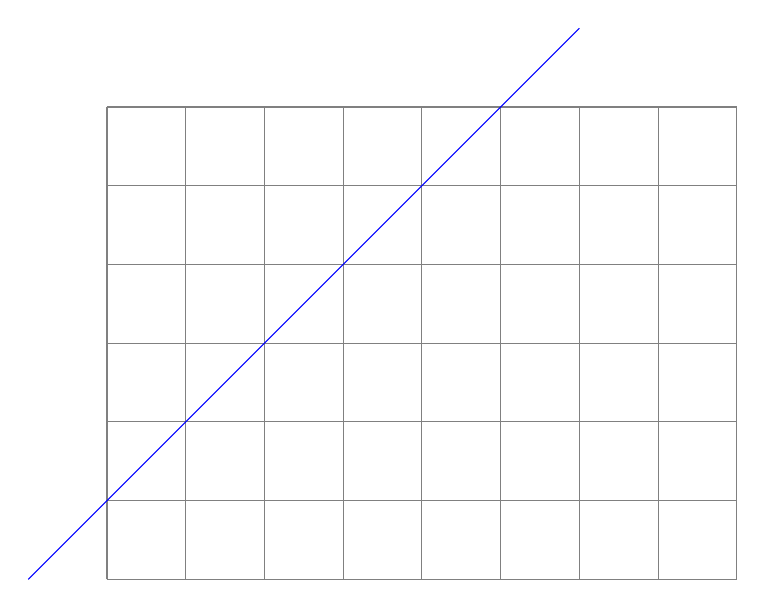
\begin{tikzpicture}
   \tkzInit[xmax=8,ymax=6]
   \tkzGrid
   \tkzAxeXY
   \draw[blue](-1,0)--(6,7);
\end{tikzpicture}
\end{tkzexample}
%<–––––––––––––––––––––––––––––––––––––––––––––––––––––––––––––––––––––––––––>

\subsubsection{Role of \tkzname{xstep} , \tkzname{ystep}}

\tkzHandBomb\   Warning, a graduation is represented by 1 cm, unless you resize the figure with the \tkzname{scale} option. In the example below \tkzname{xstep} = 2 corresponds to 1 cm, so between 0 and 10, we will need 5 cm. Similarly \tkzname{ystep}=400, so between 0 and 800 there are 2 cm. It is not possible to use the options of \TIKZ, \tkzname{x=...} and \tkzname{y=...}.

\medskip
\begin{tkzexample}[latex=7cm,small]

\begin{tikzpicture}
  \tkzInit[xmax=10,xstep=2,ymax=800,ystep=400]
  \tkzGrid  
  \tkzAxeXY 

\end{tikzpicture}
\end{tkzexample} 

\subsection{Another example with \tkzname{xstep} and \tkzname{ystep}}    
\begin{tkzexample}[latex=7cm,small]

\begin{tikzpicture}
  \tkzInit[xmax=5,xstep=1,ymax=2,ystep=.5]
    \tkzGrid  
    \tkzAxeXY 
\end{tikzpicture}
\end{tkzexample}

\subsubsection{Customized origin.}
It is important to note that you can place a point without calculating anything.
\begin{tkzexample}[latex=10cm,small]
\begin{tikzpicture}
  \tkzInit[xmin=20,
           xmax=50,
           xstep=10,
           ymin=5000,
           ymax=5150,
           ystep=50]
  \tkzAxeXY  
  \tkzDefPoint(30,5100){A}
  \tkzDrawPoint(A)  
\end{tikzpicture}
\end{tkzexample}

\subsubsection{Use of decimals }

\medskip
It is preferable to write the different arguments relating to an axis with the same number of decimals.
\tkzname{numprint} is used to display the graduations correctly.

In the following example, \tkzname{numprint} uses the English conventions for writing numbers because I used:
 
\tkzcname{usepackage[english]\{babel\} }

\medskip

\begin{tkzexample}[small]
\begin{tikzpicture}
  \tkzInit[xmin=0.00,  xmax=0.05, 
           ymin=1.2200,ymax=1.2215,
           xstep=0.01, ystep=0.0005]
  \tkzAxeXY
  \tkzDefPoint(.04,1.22025){I}
  \tkzDrawPoint(I)   
\end{tikzpicture}
\end{tkzexample}

\subsubsection{Negative values}
\begin{tkzexample}[latex=7cm,small]
\begin{tikzpicture}
  \tkzInit[xmin  = -40,
           xmax  =  60,
           ymin  = -40,
           ymax  =  60,
           xstep =  20,
           ystep =  20]
  \tkzAxeXY  
\end{tikzpicture}
\end{tkzexample}

\endinput

\section{Macros for the axes}

 \tkzHandBomb\ Careful, these macros have been modified. It's now easier to use the styles of \TIKZ. \tkzcname{tkzDrawX} allows to draw an axis, \tkzcname{tkzLabelX} places graduations and finally in simple cases \tkzcname{tkzAxeX} traces and graduations. The options of \TIKZ\ are accessible. 
Fractions can be used for graduations.
%<--------------------------------------------------------------------->
%                  tkzDrawX
%<--------------------------------------------------------------------->
\subsection{\tkzcname{tkzDrawX}} \hypertarget{dx}{}
\begin{NewMacroBox}{tkzDrawX}{\oarg{local options}}%
This macro allows you to draw the abscissa axis with default ticks.
The options are those of \TIKZ\ plus the following ones:

\medskip
\begin{tabular}{lll}%
\toprule
options  & default & definition   \\
\midrule
\TOline{color}      {black}  {Axis and ticks}
\TOline{noticks}    {false}  {no ticks on axis}
\TOline{right space}{0.5 cm} {axis extended right}
\TOline{left space} {0 cm}   {extension of the axis to the left}
\TOline{label}      {$x$}    {label name}
\TOline{trig}       {0}      {if <>0 graduations are multiples of $pi$/trig"   "trig is an integer"}
\TOline{tickwd}     {0.8pt}  {tick thickness}
\TOline{tickup}     {1pt}    {tick over axis}
\TOline{tickdn}     {1pt}    {tick depth over axis}
\bottomrule
\end{tabular}

\medskip
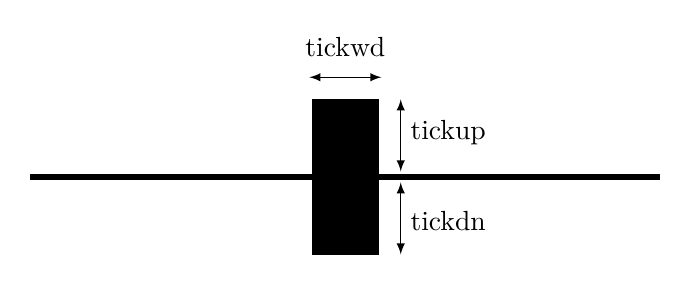
\begin{tikzpicture}[>=latex,scale=2]
  \draw[line width=2 pt](0,0)--(4,0);
  \draw[fill] (2cm-6pt,-14pt) rectangle (2cm+6pt,+14pt);
  \draw[<->](2cm-6.5pt,18pt) -- (2cm+6.5pt,+18pt);
  \node[above] at (2cm,20pt) {tickwd};
  \draw[<->](2cm+10pt,1pt) -- (2cm+10pt,+14pt);
  \node[right] at (2cm+10pt,8pt) {tickup};
  \draw[<->](2cm+10pt,-1pt) -- (2cm+10pt,-14pt);
  \node[right] at (2cm+10pt,-8pt) {tickdn};
\end{tikzpicture}

\medskip
This macro is used to draw the abscissa axis. The most important thing is to test all the options. Above, you have the values that define a tick. Otherwise the options of \TIKZ\ apply and in particular \tkzname{text}, \tkzname{color}, \tkzname{fill} and \tkzname{font}. 
\end{NewMacroBox}

\subsubsection{No tick, no label}
\begin{tkzexample}[latex=8cm,small]
\begin{tikzpicture}
 \tkzInit[xmax=5]
 \tkzDrawX[label={},noticks]
\end{tikzpicture}
\end{tkzexample}

\subsubsection{Label placement}
\begin{tkzexample}[latex=8cm,small]
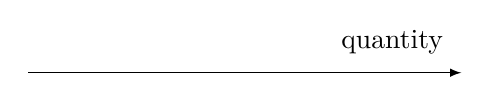
\begin{tikzpicture}
 \tkzInit[xmax=5]
 \tkzDrawX[label      = quantity,
           above left = 8pt]
\end{tikzpicture}
\end{tkzexample}


\subsubsection{Label and Axis Colour}
The color of the label is obtained with the option \tkzname{text}, that of the axis with the option \tkzname{color}.

The option \tkzname{right=12pt} shifts the label $x$ by 12 pt.

\begin{tkzexample}[latex=7cm,small]
\begin{tikzpicture}
  \tkzInit[xmax=5]
  \tkzDrawX[text=blue,color=red,right=12pt]
\end{tikzpicture}
\end{tkzexample}

\subsubsection{Option \tkzname{right space}}
It adds a little space after the last tick.
\begin{tkzexample}[latex=6cm,small]
\begin{tikzpicture}
\tkzInit[xmax=0.4,xstep=0.1]
\tkzDrawX[text=blue,color=red,right=12pt,right space=1]
\end{tikzpicture}
\end{tkzexample}

 \subsubsection{Trigonometric axis with the option \tkzname{trig=$n$}}\hypertarget{newm}{}
If $number=0$ then the axis is graduated from cm to cm, otherwise the axis is graduated using multiples of $\frac{\pi}{number}$.

\begin{tkzexample}[latex=6cm,small]
\begin{tikzpicture}
  \tkzInit[xmin=0,xmax=4,ymin=-1,ymax=1]
  \tkzDrawX[trig=1]
\end{tikzpicture}
\end{tkzexample}

\subsubsection{Trigonometric axis with the option \tkzname{trig=2} }

\begin{tkzexample}[latex=6cm,small]
\begin{tikzpicture}
  \tkzInit[xmin=0,xmax=4,ymin=-1,ymax=1]
  \tkzDrawX[trig=2]
\end{tikzpicture}
\end{tkzexample}
%<--------------------------------------------------------------------->
%                  tkzLabelX
%<--------------------------------------------------------------------->
\subsection{\tkzcname{tkzLabelX}}\hypertarget{lx}{}
\begin{NewMacroBox}{tkzLabelX}{\oarg{local options}}%
This macro allows you to place graduations. The option \tkzname{orig} can be used again, but its behavior is reversed. By default, the original value is placed.
The options are those of \TIKZ, plus the following ones:

\medskip
\begin{tabular}{lll}
\toprule
options  & default & definition   \\
\midrule
\TOline{frac}  {0}{if <>0  graduations  are multiples num/frac "frac is an integer"}
\TOline{trig}  {0}{if <>0  graduations are multiples $pi$/trig  "trig is an integer"}
\TOline{font} {\BS textstyle} {scale size.}
\TOline{color}  {black} {graduation color}
\TOline{step}  {1} {interval between graduations}
\TOline{np off}  {false} {numprint deactivation}
\TOline{orig}  {true} {displays the origin graduation }
\bottomrule
\end{tabular}

{\tkzname{frac} and \tkzname{trig} are integers that can be changed to fractional or trigonometric writing. }
\end{NewMacroBox}

\subsubsection{Position of the graduations}
\begin{tkzexample}[latex=6cm,small]
\begin{tikzpicture}
\tkzInit[xmax=.5,xstep=0.1]
\tkzDrawX[label=$t$,text=blue,color=red]
\tkzLabelX[text=blue,below = 3pt]
\end{tikzpicture}
\end{tkzexample}


\subsubsection{Position of the graduations with \tkzname{xlabel style}}
\begin{tkzexample}[latex=5cm,small]
\begin{tikzpicture}
 \tkzInit[xmin=1000,xmax=4000,xstep=1000]
 \tkzDrawX
 \tikzset{xlabel style/.append style={rotate=-30}}
 \tkzLabelX[below right=3 pt,inner sep = 1pt]
\end{tikzpicture}
\end{tkzexample}

\subsubsection{Dates with \tkzname{np off}}
For dates, you have to deactivate numprint.
\begin{tkzexample}[latex=5cm,small]
\begin{tikzpicture}
 \tkzInit[xmin=2000,xmax=2004]
 \tkzDrawX
 \tikzset{xlabel style/.append style={rotate=-30}}
 \tkzLabelX[np off,below right=3 pt,inner sep =1pt]
\end{tikzpicture}
\end{tkzexample}

\subsubsection{\tkzname{frac}}
\begin{tkzexample}[latex=6cm,small]
\begin{tikzpicture}
\tkzInit[xmax=1.75,xstep=0.33333]
\tkzDrawX[label=$t$,text=blue,color=red]
\tkzLabelX[frac=3,text=blue,below = 6pt]
\end{tikzpicture}
\end{tkzexample}

\subsubsection{\tkzname{trig}}
\begin{tkzexample}[latex=6cm,small]
\begin{tikzpicture}
  \tkzInit[xmin=0,xmax=5,ymin=-1,ymax=1]
  \tkzDrawX[trig=2]
  \tkzLabelX[trig=2,text=blue,below = 8pt]
\end{tikzpicture}
\end{tkzexample}

\subsubsection{Graduations size}
Two possibilities. It is possible to define the default style used for the math mode:

\begin{tkzltxexample}[small]
\let\tkzmathstyle\textstyle
\end{tkzltxexample}

\begin{tkzexample}[latex=6cm,small]
\begin{tikzpicture}
  \tkzInit[xmin=0,xmax=5,ymin=-1,ymax=1]
  \tkzDrawX[trig=2]
  \tkzLabelX[trig=2,text=blue,below = 8pt]
\end{tikzpicture}
\end{tkzexample}

\begin{tkzexample}[latex=6cm,small]
\begin{tikzpicture}
  \tkzInit[xmin=0,xmax=5,ymin=-1,ymax=1]
  \let\tkzmathstyle\textstyle
  \tkzDrawX[trig=2]
  \tkzLabelX[trig=2,text=blue,
            below = 8pt]
\end{tikzpicture}
\end{tkzexample}

\begin{tkzexample}[latex=6cm,small]
\begin{tikzpicture}
  \tkzInit[xmin=0,xmax=5,ymin=-1,ymax=1]
  \tkzDrawX[trig=2]
  \tkzLabelX[trig=2,text=blue,
           below = 8pt,node font=\small]
\end{tikzpicture}
\end{tkzexample}

\begin{tkzexample}[latex=6cm,small]
\begin{tikzpicture}
  \tkzInit[xmin=0,xmax=5,ymin=-1,ymax=1]
  \tkzDrawX[trig=2]
  \tkzLabelX[trig=2,text=blue,
      below = 8pt,node font=\scriptsize]
\end{tikzpicture}
\end{tkzexample}

\subsubsection{Colour of the graduations}
The key here is to use the color, text, and text options correctly. 
\begin{tkzexample}[latex=7cm,small]
\begin{tikzpicture}
  \tkzInit[xmin = -2,xmax = 3,
           ymin = -2,ymax = 2]
 \tkzDrawX[color = red,
           label = $\displaystyle\frac{1}{t}$,
           below = 6pt]
 \tkzLabelX[text=blue]
\end{tikzpicture}
\end{tkzexample}

\subsubsection{Axis drawings before the graduation}
In some cases, it is preferable to place \tkzcname{tkzDrawXY} after \tkzcname{tkzLabelX} and \tkzcname{tkzLabelY}. 

This prevents display problems.


\begin{tkzexample}[latex=7cm,small]
\begin{tikzpicture}
\tkzInit[xmin = -1,xmax = 4,
         ymin = -1,ymax = 1]
\tkzDrawXY \tkzLabelX  \tkzLabelY
\end{tikzpicture}
\end{tkzexample}

\subsubsection{Graduations (except originally) prior to tracings  }

\begin{tkzexample}[latex=7cm,small]
\begin{tikzpicture}
   \tkzInit[xmin = -1,xmax = 4,
            ymin = -1,ymax = 1]
   \tkzLabelX[orig=false] 
   \tkzLabelY[orig=false]
   \tkzDrawXY
\end{tikzpicture}
\end{tkzexample}

\subsubsection{Only positive graduations before drawings }

\begin{tkzexample}[latex=7cm,small]
\begin{tikzpicture}
  \tkzInit[xmin=2,ymin=2,xmax=4,ymax=4]
  \tkzLabelX \tkzLabelY
  \tkzDrawXY
\end{tikzpicture}
\end{tkzexample}

\subsubsection{No graduations at the origin }

\begin{tkzexample}[latex=7cm,small]
\begin{tikzpicture}
  \tkzInit[xmin=2,ymin=2,xmax=4,ymax=4]
  \tkzLabelX[orig]    \tkzLabelY[orig]
  \tkzDrawXY
\end{tikzpicture}
\end{tkzexample}
%<--------------------------------------------------------------------->
%                  tkzAxeX
%<--------------------------------------------------------------------->
\subsection{\tkzcname{tkzAxeX}}\hypertarget{ax}{}
\begin{NewMacroBox}{tkzAxeX}{\oarg{local options}}%
This macro allows you to draw the abscissa axis with default ticks as well as the graduations. It combines the two macros \tkzcname{tkzDrawX} and \tkzcname{tkzLabelX}. It should only be used in simple cases. 

\medskip
\begin{tabular}{lll}%
\toprule
options  & default & definition   \\
\midrule
\TOline{label} {$x$}{label name}
\TOline{trig} {0}{if <>0, graduations are multiples of $pi$/trig}
\TOline{frac} {0}{if <>0, graduations are multiples of 1/frac}
\TOline{swap} {false}{allows you to run \tkzcname{tkzLabelX} before \tkzcname{tkzDrawX}}
\bottomrule
\end{tabular}

The option \tkzname{text} defines the color of the graduations.
\end{NewMacroBox}

\subsubsection{Example with \tkzcname{tkzAxeX}}
\begin{tkzexample}[latex=7cm,small]

\begin{tikzpicture}
   \tkzInit[xmax=0.5,xstep=0.1,ymax=1]
   \tkzGrid
   \tkzAxeX[text=blue]
\end{tikzpicture}
\end{tkzexample}

\subsubsection{Use of \tkzname{pi} and \tkzcname{tkzAxeX}}
\begin{tkzexample}[latex=5cm,small]
\begin{tikzpicture}
  \tkzInit[xmax=4,ymax=3.5]
  \let\tkzmathstyle\displaystyle
  \tkzLabelX[orig  = false, frac  = 4,below = 10pt]
  \tkzDrawX[label = $t$]
  \tkzAxeY[trig=2]
\end{tikzpicture}
\end{tkzexample}


\subsubsection{Option \tkzname{frac} and \tkzname{trig}}
In this example, we position the $t$ label as well as the graduations.  \tkzcname{below=10pt} is used to place the graduations underneath.
\begin{tkzexample}[latex=5cm,small]
\begin{tikzpicture}
  \tkzInit[xmax=9,xstep=3,ymax=3.5]
  \tkzLabelX[below=10pt,orig=false,frac=3]
  \tkzDrawX[label = $t$]
  \tkzAxeY[trig=2]
\end{tikzpicture}
\end{tkzexample}

%<--------------------------------------------------------------------->
%                  tkzDrawY
%<--------------------------------------------------------------------->
\subsection{\tkzcname{tkzDrawY}} \hypertarget{dy}{}
\begin{NewMacroBox}{tkzDrawY}{\oarg{local options}}%
This macro allows you to draw the ordinate axis with default ticks.
The options are those of \TIKZ\ plus the following ones:

\medskip
\begin{tabular}{lll}%
\toprule
options  & default & definition   \\
\midrule
\TOline{color}      {black} {color of axis and ticks}
\TOline{noticks}    {false} {no ticks on the axis}
\TOline{up space}   {0.5 cm} {top axis extension}
\TOline{down space} {0 cm}{axis extension down}
\TOline{label}      {$x$}{label name}
\TOline{trig}    {0}{if <>0, graduations are multiples of $pi$/trig "trig is an integer" }
\TOline{tickwd}     {0.8pt}{tick's thickness}
\TOline{ticklt}     {1pt}{height of the tick above the axis}
\TOline{tickrt}     {1pt}{above-axis tick depth}
\end{tabular}
\end{NewMacroBox}

\subsection{\tkzcname{tkzLabelY}} \hypertarget{ly}{}
\begin{NewMacroBox}{tkzLabelY}{\oarg{local options}}%
This macro allows you to draw the abscissa axis with default ticks.
The options are those of \TIKZ\ plus the following ones:

\medskip
\begin{tabular}{lll}%
\toprule
options  & default & definition   \\
\midrule
\TOline{color}  {black} {graduation color}
\TOline{frac} {0}{if <>0, graduations are multiples of $1$/frac "frac is an integer"}
\TOline{font} {\BS textstyle} {graduation size.}
\TOline{step}  {1} {interval between graduations}
\bottomrule
\end{tabular}

{\tkzname{frac} is a integer that can be changed to fractional or trigonometric writing.}
\end{NewMacroBox}

%<--------------------------------------------------------------------->
%                  tkzAxeY
%<--------------------------------------------------------------------->
\subsection{\tkzcname{tkzAxeY}}\hypertarget{ay}{}
\begin{NewMacroBox}{tkzAxeY}{\oarg{local options}}%
This macro combines the two macros:
\tkzcname{tkzDrawY} \tkzcname{tkzLabelY}
See \tkzcname{tkzAxeX} for options.
\end{NewMacroBox}
%<--------------------------------------------------------------------->
%                  tkzAxeXY
%<--------------------------------------------------------------------->
\subsection{\tkzcname{tkzAxeXY}}  \hypertarget{axy}{}
\begin{NewMacroBox}{tkzAxeXY}{\oarg{local options}}%
This macro combines the four macros:
\tkzcname{tkzDrawX}\tkzcname{tkzDrawY} \tkzcname{tkzLabelX}\tkzcname{tkzLabelY}

It is necessary to use common options as in the example below, but this means that the same options are applied to both macros. Thus it is not possible to change \tkzname{label}.
\end{NewMacroBox}

\subsubsection{Colour of axes, graduations}

\begin{tkzexample}[latex=6cm]
\begin{tikzpicture}
  \tkzInit[xmin=-1,xmax=4,ymin=-1,ymax=3]
  \tkzAxeXY[label={},text=blue]
\end{tikzpicture}
\end{tkzexample}

\subsubsection{Option \tkzname{label=\{\}}}

\begin{tkzexample}[latex=6cm,small]
\begin{tikzpicture}
  \tkzInit[xmin=-1,xmax=4,ymin=-1,ymax=2]
  \tkzAxeXY[label={},text=blue,trig=2]
\end{tikzpicture}
\end{tkzexample}

\subsubsection{Option \tkzname{swap}}
\begin{tkzexample}[latex=6cm,small]
\begin{tikzpicture}
\tkzInit[xmin=-2,xmax=2,ymin=-2,ymax=2]
\tkzAxeXY[label={},swap]
\end{tikzpicture}
\end{tkzexample}
%<--------------------------------------------------------------------->
%                  tkzDrawXY
%<--------------------------------------------------------------------->
\subsection{\tkzcname{tkzDrawXY}}  \hypertarget{dxy}{}
\begin{NewMacroBox}{tkzDrawXY}{\oarg{local options}}%
This macro combines the two macros: \tkzcname{tkzDrawX}\tkzcname{tkzDrawY}.
It is necessary to use common options as in the example below.
\end{NewMacroBox}

\subsubsection{Common colour and empty labels}
\begin{tkzexample}[latex=6cm,small]
\begin{tikzpicture}
   \tkzInit[xmin=-1,xmax=4,ymin=-1,ymax=1]
   \tkzDrawXY[label={},color=red]
\end{tikzpicture}
\end{tkzexample}

\subsubsection{Two trigonometric axes}
\begin{tkzexample}[latex=6cm,small]
\begin{tikzpicture}
  \tkzInit[xmin=-1,xmax=4,ymin=-1,ymax=1]
  \tkzDrawXY[label={},color=red,trig=4]
\end{tikzpicture}
\end{tkzexample}
%<--------------------------------------------------------------------->
%                  tkzLabelXY
%<--------------------------------------------------------------------->
\subsection{\tkzcname{tkzLabelXY}}  \hypertarget{lxy}{}
\begin{NewMacroBox}{tkzLabelXY}{\oarg{local options}}%
This macro combines the two macros:

 \tkzcname{tkzLabelX}\tkzcname{tkzLabelY}

It is necessary to use common options as in the example below.
\end{NewMacroBox}

\subsubsection{}
\begin{tkzexample}[latex=6cm,small]
\begin{tikzpicture}
  \tkzInit[xmin=-1,xmax=4,ymin=-1,ymax=1]
  \tkzDrawXY[label={},color=red]
  \tkzLabelXY[text=blue]
\end{tikzpicture}
\end{tkzexample}

%<--------------------------------------------------------------------->
%                  tkzSetUpAxis
%<--------------------------------------------------------------------->
\subsection{Changing values by axis default} \hypertarget{axis}{}

\begin{NewMacroBox}{tkzSetUpAxis}{\oarg{local options}}%
\begin{tabular}{lll}%
options  & default & definition   \\
\midrule
\TOline{line width}{|0.4pt|}{line width defines the width of the line}
\TOline{tickwd}{|0.8pt|}{tick thickness  }
\TOline{ticka}{|1pt|}{right side or above the tick  }
\TOline{tickb}{|1pt|}{left side or below the tick  }
\TOline{font}{|\tkzcname{textstyle}|}{graduation size.}
\end{tabular}
\end{NewMacroBox}

\subsubsection{Changing the default axes}
\begin{tkzexample}[latex=5cm,small]
\begin{tikzpicture}[scale=1]
 \tkzInit[ymax=2,xmax=4]
 \tkzSetUpAxis[line width=1pt,tickwd=1pt,ticka=3pt, tickb=0pt]
 \tkzAxeXY
\end{tikzpicture}
\end{tkzexample}

You have to run \tkzcname{tkzSetUpAxis} again to retrieve the default values.

\medskip
\begin{tkzltxexample}[small]
\tkzSetUpAxis[line width=1pt,tickwd=1pt,ticka=2pt,tickb=2pt]
\end{tkzltxexample}

\tkzSetUpAxis[line width=1pt,tickwd=1pt,ticka=2pt,tickb=2pt]

\endinput

\section{Use of \tkzcname{tkzGrid}} \hypertarget{grid}{}   

\begin{NewMacroBox}{tkzGrid}{\oarg{local options}\parg{$x_A~;~y_A$} \parg{$x_B~;~y_B$}}%
A few changes for this macro. First of all, to simplify currently the color of the thinnest grid is determined automatically from the main grid, same process for the thickness.  This behavior can be modified using styles. 

\begin{tabular}{lll}%
options   & default & definition                                        \\
\midrule  
\TAline{\parg{$x_A~;~y_A$} \parg{$x_B~;~y_B$}}{(xmin,ymin)(xmax,ymax)} {grid pattern} 
\end{tabular}  
 
\begin{tabular}{lll}%
options   & default & definition                                        \\
\midrule  
\TOline{sub}{true} {asks for a sub-grid }
\TOline{color}{darkgray}{main grid color}
\TOline{subxstep}{0.2} {the step of the subgraduations for the abscissa axis}  
\TOline{subystep}{0.2}{the step of the subgraduations for the ordinate axis } 
\TOline{line width}{0.4pt} {main grid line thickness} 
\bottomrule  
\end{tabular}

\medskip
Default values can be changed in the configuration file or by macros. The color of the second grid is the same as the main grid, but less intense (by default |gray!50|). 

Same behavior for the line thickness (by default |0.75 of line width|). See the examples to change this behavior.
\end{NewMacroBox}  

\subsubsection{\tkzcname{tkzGrid} and the option \tkzname{sub}}
The option \tkzname{sub} allows you to display a finer secondary grid.
It is preferable to run \tkzcname{tkzGrid} first,
 to prevent the grid from being overlapped with other elements.
\begin{tkzexample}[latex=8cm,small]

\begin{tikzpicture}
 \tkzInit[xmax=4, ymax=2]
 \tkzGrid[sub] 
 \tkzAxeXY    
\end{tikzpicture}
\end{tkzexample}  

\subsubsection{Option \tkzname{sub}}
The option \tkzname{sub} allows to display a finer secondary grid. Some parameters are modifiable.

\begin{tkzexample}[latex=6cm,small] 
\def\tkzCoeffSubColor{20}% instead of 50
\def\tkzCoeffSubLw{0.2}% instead of 0.75 

\begin{tikzpicture}
 \tkzInit[xmax=4, ymax=2]
 % we can change the step for the second grid 
 \tkzGrid[sub,color=orange,
         subxstep=.5,subystep=.5] 
  \tkzAxeXY 
\end{tikzpicture}
\end{tkzexample}    

\subsubsection{Almost Default}
\begin{tkzexample}[width=7cm,small]

\begin{tikzpicture}
  \tkzInit[xmax=5,ymax=2]
  \tkzGrid[color=orange]
  \tkzAxeXY  
\end{tikzpicture}
\end{tkzexample}

\subsubsection{Under the grid, too, option \tkzname{sub}}
\begin{tkzexample}[width=7cm,small]
 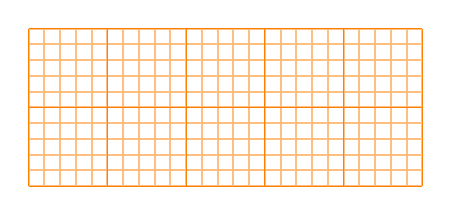
\begin{tikzpicture}
  \tkzInit[xmax=5,ymax=2]
  \tkzGrid[sub,color=orange]
  \tkzGrid[color=orange]
  \tkzAxeXY  
 \end{tikzpicture}
\end{tkzexample}

\subsubsection{Grid change}
\begin{tkzexample}[width=7cm,small]
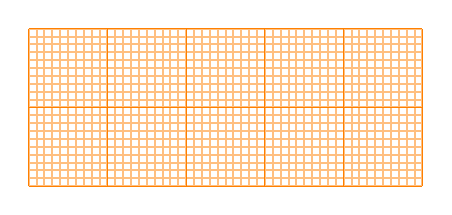
\begin{tikzpicture}
  \tkzInit[xmax=5,ymax=2]
  \tkzGrid[color    = orange,
           sub,
           subxstep = 0.1,
           subystep = 0.1] 
   \tkzAxeXY 
\end{tikzpicture}
\end{tkzexample}
 
\subsubsection{Option \tkzname{xstep}, \tkzname{xstep}, \tkzname{subxstep} and \tkzname{subystep}}
\begin{tkzexample}[latex=7cm,small]

\begin{tikzpicture}
\tkzInit[xmax=.5,xstep=.1,
         ymax=.2,ystep=.1]
\tkzGrid[sub,
         subxstep = 0.05,
         subystep = 0.05,
         color=orange]
\tkzAxeXY 
\end{tikzpicture} 
\end{tkzexample}

\subsubsection{With large intervals}
\begin{tkzexample}[width=7cm,small]
\begin{tikzpicture}
   \tkzInit[xmax=100,xstep=20,
            ymax=3000,ystep=1000]
   \tkzGrid[sub,subxstep=10,
                subystep=500,
                color=orange]
   \tkzAxeXY 
\end{tikzpicture}
\end{tkzexample}

\subsubsection{\tkzcname{tkzGrid} and the arguments}  
The grid can be any size.
\begin{tkzexample}[width=8cm,small]
\begin{tikzpicture}
   \tkzInit[xmax=100,xstep=20,
            ymax=3000,ystep=1000]
   \tkzGrid[sub,subxstep=10,
            subystep=500,
            color=orange]
            (-20,-1000)(115,4000)%
  \tkzAxeXY 
\end{tikzpicture}
\end{tkzexample} 

\subsubsection{Use of \tkzname{pi} with \tkzcname{tkzGrid}} 
\begin{tkzexample}[width=8cm,small]   
\begin{tikzpicture}[scale=.75] 
   \tkzInit[xmax=6.5,ymax=6.5]
   \tkzGrid[xstep=pi,ystep=pi/2,sub,
            subxstep=pi/4,subystep=pi/4]
   \tkzLabelX[label=$t$,orig=false,trig=4,
            below=6pt,font=\scriptsize]
   \tkzLabelY[trig=2,font=\scriptsize]
   \tkzDrawXY  
\end{tikzpicture}  
\end{tkzexample}  

\subsubsection{Options \tkzname{frac} and \tkzname{trig} with \tkzcname{tkzGrid}}
\begin{tkzexample}[width=8cm,small]   
\begin{tikzpicture} 
   \tkzInit[xmax=9,xstep=3,ymax=4]
   \tkzGrid[xstep=1,ystep=pi/2,sub,
            subxstep=1,subystep=pi/4]
   \tkzLabelX[label=$t$,orig=false,frac=3,
            below=6pt,font=\scriptsize]
   \tkzLabelY[trig=2,font=\scriptsize]
\end{tikzpicture}
\end{tkzexample}

\subsubsection{Use of a repetition grid}
\begin{tkzexample}[latex=8cm,small] 
\begin{tikzpicture}[scale=.5]
 % \tikzset{xaxe style/.style ={-}} 
  \tkzInit[xmax=15,ymax=15]
  \tkzClip 
  \tkzGrid[sub,color=orange] 
  \tkzLabelX[label= ]   \tkzLabelY[label= ]
  \tkzDrawXY   
  \node[opacity=.5] at (8,6){%
    
\includegraphics[scale=.5]{tiger}};
\end{tikzpicture}
\end{tkzexample}

                
\endinput

\section{The points}

I made a distinction between the point used in Euclidean geometry and the point used to represent an element of a statistical cloud. In the first case, I use as object a \tkzname{node}, which means that the representation of the point cannot be modified by a \tkzname{scale}; in the second case, I use as object a \tkzname{plot mark}. The latter can be scaled and have more varied forms than the node.

The new macro is \tkzNameMacro{tkzDefPoint}, it allows to use \TIKZ-specific options as a shift and the values are processed with tkz-base. Moreover, if calculations are needed then the \tkzNamePack{xfp} package takes care of them. You can use Cartesian or polar coordinates.

\subsection{Defining a point in Cartesian coordinates: \tkzcname{tkzDefPoint}} \hypertarget{tdp}{}

\begin{NewMacroBox}{tkzDefPoint}{\oarg{local options}\parg{x,y}\var{name} or \parg{a:r}\var{name}}%
\begin{tabular}{lll}%
arguments &  default & definition  \\ 
\midrule
\TAline{x,y}{no default}{$x$ and $y$ are two dimensions, by default in cm.}
\TAline{a:r}{no default}{$a$ is an angle in degrees, $r$ is a dimension}
\bottomrule
\end{tabular}

\medskip
\noindent{The mandatory arguments of this macro are two dimensions expressed with decimals, in the first case they are two measures of length, in the second case they are a measure of length and the measure of an angle in degrees}.

\medskip
\begin{tabular}{lll}%
\toprule
options             & default & definition   \\ 
\midrule
\TOline{shift} {(0,0)} {value spacing}
 \bottomrule
\end{tabular}

\medskip
\noindent{All the options of \TIKZ\ that we can apply to \tkzname{coordinate}, are applicable (well I hope!) as for example the option \tkzname{label} defined with the library \tkzname{quotes}.}
\end{NewMacroBox}

\subsubsection{Use of \tkzname{shift}}
\tkzname{shift} allows the points to be placed in relation to each other. 

\begin{tkzexample}[latex=7cm,small]
\begin{tikzpicture}[trim left=-1cm]
 \tkzDefPoint(2,3){A}
 \tkzDefPoint[shift={(2,3)}](31:3){B}  
 \tkzDefPoint[shift={(2,3)}](158:3){C}
 \tkzDrawSegments[color=red,line width=1pt](A,B A,C) 
 \tkzDrawPoints[color=red](A,B,C)
\end{tikzpicture}
\end{tkzexample}

\subsection{Placing a label with the library \tkzname{quotes}}
I prefer not to mix operations and use \tkzcname{tkzLabelPoint} to place labels. See the section "The  Quotes Syntax" in the \TIKZ\ manual.

\begin{tkzexample}[latex=7cm,small]
\begin{tikzpicture}[trim left=-1cm]
 \tkzDefPoint["-60:$A_n$" ](2,3){A}
 \tkzDefPoint[shift={(2,3)},%
    "$B_n$" above left](31:3){B}  
 \tkzDefPoint[shift={(2,3)},%
     "$C_n$" above right](158:3){C}
 \tkzDrawSegments[color=red,%
          line width=1pt](A,B A,C) 
 \tkzDrawPoints[color=red](A,B,C)
\end{tikzpicture}
\end{tkzexample}


\subsubsection{Rotation with \tkzname{shift} and \tkzname{scope}}  
Preferable to rotate is to use a \tkzNameEnv{scope} environment. 
                    
\begin{tkzexample}[latex=7cm,small] 
\begin{tikzpicture}[scale=.75,rotate=90] 
 \tkzDefPoint[label=right:$A_n$](2,3){A} 
 \begin{scope}[shift={(A)}]
   \tkzDefPoint[label= right:$B_n$](31:3){B} 
   \tkzDefPoint[label= right:$C_n$](158:3){C} 
 \end{scope}
  \tkzDrawSegments[color=red,%
           line width=1pt](A,B A,C) 
  \tkzDrawPoints[color=red](A,B,C)
 \end{tikzpicture}
\end{tkzexample}

\subsubsection{Forms and coordinates}
Here we must follow the syntax of \tkzNamePack{xfp}. It is always possible to go through \tkzNamePack{pgfmath} but in this case, the coordinates must be calculated before using the macro \tkzcname{tkzDefPoint}.

\begin{tkzexample}[latex=6cm,small]
\begin{tikzpicture}[scale=.75]
  \tkzInit[xmax=6,ymax=6]
  \tkzGrid
  \tkzSetUpPoint[shape = circle,color = red,%
                 size = 4,fill = red!30]
  \tkzDefPoint(-1+1,-1+4){O}
  \tkzDefPoint({3*ln(exp(1))},{exp(1)}){A}
  \tkzDefPoint({4*sin(pi/6)},{4*cos(pi/6)}){B}
  \tkzDefPoint({4*sin(pi/3)},{4*cos(pi/3)}){B'}
  \tkzDefPoint[shift={(1,3)}](30:3){A'} 
  \tkzDrawPoints(O,A,B) 
  \tkzDrawPoints[color=red,shape=cross out](B',A') 
  \tkzLabelPoints(A,O,B,B',A') 
\end{tikzpicture}
\end{tkzexample}

\subsubsection{Scope and \tkzcname{tkzDefPoint}}
First, we can use the \tkzNameEnv{scope} of \TIKZ. 
In the following example, we have a way to define an isosceles triangle.

\begin{tkzexample}[latex=7cm,small]
\begin{tikzpicture}[scale=1]
 \begin{scope}[rotate=30]
  \tkzDefPoint(2,3){A}
  \begin{scope}[shift=(A)]
     \tkzDefPoint(90:5){B}
     \tkzDefPoint(30:5){C}
  \end{scope}
 \end{scope}
\tkzDrawSegments[color=blue](A,B B,C C,A) 
\tkzDrawPoints(A,B,C)
\tkzLabelPoints[above](B,C)
\tkzLabelPoints[below](A) 
\end{tikzpicture}
\end{tkzexample}
%<--------------------------------------------------------------------------->
\subsection{Definition of points in Cartesian coordinates: \tkzcname{tkzDefPoints}} \hypertarget{tdps}{} 
 
\begin{NewMacroBox}{tkzDefPoints}{\oarg{local options}\var{$x_1/y_1/n_1,x_2/y_2/n_2$, ...}}%
$x_1$ and $y_1$ are the coordinates of a referenced point $n_1$ 

\begin{tabular}{lll}%
\toprule
arguments &  example  &   \\ 
\midrule
\TAline{$x_i/y_i/n_i$}{\tkzcname{tkzDefPoints\{0/0/O,2/2/A\}}}{}
\end{tabular}
\end{NewMacroBox}

\subsubsection{Definition of points}
\begin{tkzexample}[latex=6cm,small]
\begin{tikzpicture}[scale=1]
 \tkzDefPoints{0/0/A,2/0/B,2/2/C,0/2/D}
 \tkzDrawSegments(D,A A,B B,C C,D)
 %with tkz-euclide \tkzDrawPolygon(A,...,D)
 \tkzDrawPoints(A,B,C,D) 
\end{tikzpicture}
\end{tkzexample}   

%<--------------------------------------------------------------------------->
\subsection{Point relative to another: \tkzcname{tkzDefShiftPoint}} 
\hypertarget{tdsp}{} 
\begin{NewMacroBox}{tkzDefShiftPoint}{\oarg{Point}\parg{x,y}\var{name} ou \parg{a:r}\var{name}}%
\begin{tabular}{lll}%
arguments &  default & definition \\ 
\midrule
\TAline{(x,y)}{no default}{$x$ and $y$ are two dimensions, by default in cm.}
\TAline{(a:r)}{no default}{$a$ is an angle in degrees, $r$ is a dimension}
\TAline{point} {no default} {\tkzcname{tkzDefShiftPoint}[A](0:4)\{B\}} 
\bottomrule
\end{tabular}

No options. The name of the point is mandatory.
\end{NewMacroBox}

\subsubsection{Example with  \tkzcname{tkzDefShiftPoint}}
This macro allows you to place one point relative to another. This is equivalent to a translation. Here is how to construct an isosceles triangle with main vertex $A$ and angle at vertex of $30^\circ$. 

\begin{tkzexample}[latex=7cm,small]
\begin{tikzpicture}[rotate=-30]
 \tkzDefPoint(2,3){A}
 \tkzDefShiftPoint[A](0:4){B}
 \tkzDefShiftPoint[A](30:4){C} 
 \tkzDrawSegments(A,B B,C C,A)
 \tkzMarkSegments[mark=|,color=red](A,B A,C)
 \tkzDrawPoints(A,B,C) 
 \tkzLabelPoints[above](A,C)   
 \tkzLabelPoints(B) 
\end{tikzpicture}
\end{tkzexample}

\subsection{Point relative to another: \tkzcname{tkzDefShiftPointCoord}}
\begin{NewMacroBox}{tkzDefShiftPointCoord}{\oarg{a,b}\parg{x,y}\var{name} or \parg{a:r}\var{name}}%
{This involves performing a $(a,b)$ vector translation at the defined point relative to the origin.}

\medskip
\begin{tabular}{lll}%
\toprule
arguments &  default & definition \\ 
\midrule
\TAline{(x,y)}{no default}{$x$ and $y$ are two dimensions, by default in cm.}
\TAline{(a:r)}{no default}{$a$ is an angle in degrees, $r$ is a dimension}
\bottomrule
\end{tabular}

\medskip
\begin{tabular}{lll}%
options             & default & example   \\ 
\midrule
\TOline{a,b} {no default} {\tkzcname{tkzDefShiftPointCoord}[2,3](0:4)\{B\}}
 \bottomrule
\end{tabular}

The option is mandatory
\end{NewMacroBox}

  
\subsubsection{Equilateral triangle with \tkzcname{tkzDefShiftPointCoord}}
Let's see how to get an equilateral triangle (there is much simpler)

\begin{tkzexample}[latex=7cm,small]
\begin{tikzpicture}[scale=1]
 \tkzDefPoint(2,3){A}
 \tkzDefShiftPointCoord[2,3](30:4){B}
 \tkzDefShiftPointCoord[2,3](-30:4){C} 
 \tkzDrawSegments(A,B B,C C,A) 
 % or \tkzDrawPolygon
  \tkzDrawPoints(A,B,C)
  \tkzLabelPoints(B,C)  
  \tkzLabelPoint[left](A){$A$} 
\end{tikzpicture}
\end{tkzexample} 

\subsubsection{Isosceles triangle with \tkzcname{tkzDefShiftPointCoord}}
Let's see how to obtain an isosceles triangle with a principal angle of 30 degrees. Rotation is possible. $AB=AC=5$ and $\widehat{BAC}$

\begin{tkzexample}[latex=7cm,small]
\begin{tikzpicture}[rotate=15]
 \tkzDefPoint(2,3){A}
 \tkzDefShiftPointCoord[2,3](15:5){B}
 \tkzDefShiftPointCoord[2,3](-15:5){C} 
 \tkzDrawSegments(A,B B,C C,A) 
 \tkzDrawPoints(A,B,C)
 \tkzLabelPoints(B,C)
 \tkzLabelPoint[left](A){$A$}
\end{tikzpicture}
\end{tkzexample}

%<--------------------------------------------------------------------------->
\subsection{Drawing a point \tkzcname{tkzDrawPoint}} \hypertarget{tdrp}{}
\begin{NewMacroBox}{tkzDrawPoint}{\oarg{local options}\parg{point}}%
\begin{tabular}{lll}%
arguments &  default & definition                 \\ 
\midrule
\TAline{point} {no default}  {a name or reference is requested}
\bottomrule
\end{tabular}

\medskip
\noindent{The argument is mandatory, but it is not necessary (although recommended) to use a reference; a pair of coordinates placed between braces is accepted. The disk takes the color of the circle, but 50\% lighter. It is possible to modify everything. The point is a node and is therefore invariant if the drawing is modified by scaling..}

\medskip
\begin{tabular}{lll}%
\toprule
options             & default & definition  \\ 
\midrule
\TOline{shape}  {circle}{Possible \tkzname{cross} or \tkzname{cross out}} 
\TOline{size}   {2 pt} {disk size}
\TOline{color}  {black}{the default color can be changed}
\bottomrule
\end{tabular}

\medskip
\noindent{We can create other forms such as \tkzname{cross}}
\end{NewMacroBox}

\subsubsection{Default stitch style} 
\begin{tkzexample}[latex=5cm,small]
  \begin{tikzpicture}
   \tkzDefPoint(1,3){A}
   \tkzDrawPoint(A)
  \end{tikzpicture}
\end{tkzexample}  

\subsubsection{Changing the style} 
The default definition is in the file \tkzname{tkz-base.cfg}

\begin{tkzltxexample}[small]
\tikzset{point style/.style={draw         = \tkz@euc@pointcolor,
                             inner sep    = 0pt,
                             shape        = \tkz@euc@pointshape,
                             minimum size = \tkz@euc@pointsize,
                             fill         = \tkz@euc@pointcolor!50}}
\end{tkzltxexample}

\begin{tkzexample}[latex=5cm,small]
  \begin{tikzpicture}
   \tikzset{point style/.style={%
     draw         = blue,
     inner sep    = 0pt,
     shape        = circle,
     minimum size = 6pt,
     fill         = red!20}}
   \tkzDefPoint(1,3){A}
   \tkzDefPoint(4,1){B}
   \tkzDefPoint(0,0){O}
   \tkzDrawPoint(A)
   \tkzDrawPoint(B)
   \tkzDrawPoint(O)
  \end{tikzpicture} 
\end{tkzexample} 

\subsubsection{Example of point plots}
Note that \tkzname{scale} does not affect the shape of the dots. Which is normal.  Most of the time, we are satisfied with a single point shape that we can define from the beginning, either with a macro or by modifying a configuration file. 

\begin{tkzexample}[latex=5cm,small]
  \begin{tikzpicture}[scale=.5]
   \tkzDefPoint(1,3){A}
   \tkzDefPoint(4,1){B}
   \tkzDefPoint(0,0){O}
   \tkzDrawPoint[shape=cross out,size=12,color=red](A)
   \tkzDrawPoint[shape=cross,size=12,color=blue](B)
   \tkzDrawPoint[size=12,color=green](O)
   \tkzDrawPoint[size=12,color=blue,fill=yellow]({2,2})
  \end{tikzpicture}
\end{tkzexample}

It is possible to draw several points at once, but this macro is a little slower than the previous one. Moreover, we have to make do with the same options for all the points.                               

\subsection{Drawing points \tkzcname{tkzDrawPoints}}
\hypertarget{tdrps}{}
\begin{NewMacroBox}{tkzDrawPoints}{\oarg{local options}\parg{liste}}%
\begin{tabular}{lll}%
arguments &  default & definition \\ 
\midrule
\TAline{points list}{no default}{example \tkzcname{tkzDrawPoints(A,B,C)}}
\bottomrule
\end{tabular}

\medskip
Warning at the final "s", an oversight leads to cascading errors if you attempt to plot multiple points. The options are the same as for the previous macro. 
\end{NewMacroBox}

\subsubsection{Example with \tkzcname{tkzDefPoint} and \tkzcname{tkzDrawPoints} } 
\begin{tkzexample}[latex=7cm,small]
  \begin{tikzpicture}[scale=.5]
   \tkzDefPoint(1,3){A}
   \tkzDefPoint(4,1){B}
   \tkzDefPoint(0,0){O}
   \tkzDrawPoints[size=8,color=red](A,B,O)
  \end{tikzpicture}
\end{tkzexample} 
  
\subsubsection{More complex example } 
\begin{tkzexample}[latex=7cm]
\begin{tikzpicture}[scale=.5]
 \tkzDefPoint(2,3){A}  \tkzDefPoint(5,-1){B}  
 \tkzDefPoint[label=below:$\mathcal{C}$,
               shift={(2,3)}](-30:5.5){E}
 \begin{scope}[shift=(A)]
    \tkzDefPoint(30:5){C}
 \end{scope}   
 \tkzCalcLength[cm](A,B)\tkzGetLength{rAB}
 \tkzDrawCircle[R](A,\rAB cm)
 \tkzDrawSegment(A,B)
 \tkzDrawPoints(A,B,C) 
 \tkzLabelPoints(B,C)
 \tkzLabelPoints[above](A)
\end{tikzpicture}
\end{tkzexample}  

%<--------------------------------------------------------------------------->
\subsection{Add a label to a point \tkzcname{tkzLabelPoint}} 
\hypertarget{tlp}{}
It is possible to add several labels at the same point by using this macro several times.  

\begin{NewMacroBox}{tkzLabelPoint}{\oarg{local options}\parg{point}\var{label}}%
\begin{tabular}{lll}%
arguments &  example  &                  \\ 
\midrule
\TAline{point}{\tkzcname{tkzLabelPoint(A)\{\$A\_1\$\}}}{}
options  & default & definition\\
\midrule
\TOline{TikZ options}{}{colour, position etc.}
\bottomrule
\end{tabular}

\medskip
Optionally, we can use any style of \TIKZ, especially placement with above, right, dots...
\end{NewMacroBox}

\subsubsection{Example with \tkzcname{tkzLabelPoint}} 
\begin{tkzexample}[latex=7cm,small]  
\begin{tikzpicture}
  \tkzDefPoint(0,0){A}
  \tkzDefPoint(4,0){B}
  \tkzDefPoint(0,3){C}
  \tkzDrawSegments(A,B B,C C,A)
  \tkzDrawPoints(A,B,C)
  \tkzLabelPoint[left,red](A){$A$}
  \tkzLabelPoint[right,blue](B){$B$}
  \tkzLabelPoint[above,purple](C){$C$}  
\end{tikzpicture} 
\end{tkzexample} 

\subsubsection{Label and reference}
 The reference of a point is the object that allows to use the point, the label is the name of the point that will be displayed.
 
\begin{tkzexample}[latex=8cm,small]
 \begin{tikzpicture}
    \tkzInit[xmax=1,xstep=0.15,ymax=.5]
    \tkzAxeX \tkzDrawY[noticks]
    \tkzDefPoint(0.22,0.25){A} 
    \tkzDrawPoint(A)
    \tkzLabelPoint[above](A){$A_1$}  
  \end{tikzpicture}
 \end{tkzexample}
%<--------------------------------------------------------------------------->
\subsection{Add labels to points \tkzcname{tkzLabelPoints}}
It is possible to place several labels quickly when the point references are identical to the labels and when the labels are placed in the same way in relation to the points. By default, \tkzname{below right} is chosen.
\hypertarget{tlps}{}  

\begin{NewMacroBox}{tkzLabelPoints}{\oarg{local options}\parg{$A_1,A_2,...$}}%
\begin{tabular}{lll}
arguments &  example & result                 \\ 
\midrule
\TAline{list of points}{\tkzcname{tkzLabelPoints(A,B,C)}}{Display of $A$, $B$ and $C$}
\bottomrule
\end{tabular}

\medskip
This macro reduces the number of lines of code, but it is not obvious that all points need the same label positioning.
\end{NewMacroBox}

\subsubsection{Example with \tkzcname{tkzLabelPoints}}   
\begin{tkzexample}[latex = 7cm,small]  
\begin{tikzpicture}
  \tkzDefPoint(2,3){A}
  \tkzDefShiftPoint[A](30:2){B}
  \tkzDefShiftPoint[A](30:5){C}
  \tkzDrawPoints(A,B,C)
  \tkzLabelPoints(A,B,C) 
\end{tikzpicture} 
\end{tkzexample}
%<--------------------------------------------------------------------------->
%                       tkzAutoLabelPoints
%<--------------------------------------------------------------------------->
\subsection{Automatic position of labels \tkzcname{tkzAutoLabelPoints}}
The label of a point is placed in a direction defined by a \tkzname{center} and a point . The distance to the point is determined by a percentage of the distance between the center and the point. This percentage is given by \tkzname{dist}.
\begin{NewMacroBox}{tkzLabelPoints}{\oarg{local options}\parg{$A_1,A_2,...$}}%
\begin{tabular}{lll}
arguments &  example & result                 \\ 
\midrule
\TAline{list of points}{\tkzcname{tkzLabelPoint(A,B,C)}}{Display of $A$, $B$ and $C$}
\end{tabular}

\medskip
\begin{tabular}{lll}
options &  default & definition                 \\ 
\midrule
\TOline{center}{no default}{you need to deisgn a center}
\TOline{dist}{0.15}{percentage change in the distance between the center and the points} 
\end{tabular}
\end{NewMacroBox}

\subsubsection{Example 1 with \tkzcname{tkzAutoLabelPoints}} 
Here the points are positioned relative to the center of gravity of $A,B,C \ \text{et}\ O$.
\begin{tkzexample}[latex=5cm,small]
\begin{tikzpicture}[scale=1.25]
  \tkzDefPoint(2,1){O}
  \tkzDefRandPointOn[circle=center O radius 1.5cm]
  \tkzGetPoint{A}
  \tkzDrawCircle(O,A) 
  \tkzDefPointBy[rotation=center O angle 100](A)
  \tkzGetPoint{C}
  \tkzDefPointBy[rotation=center O angle 78](A)
  \tkzGetPoint{B}
  \tkzDrawPoints(O,A,B,C) 
  \tkzDrawSegments(C,B B,A A,O O,C)
  \tkzDefCentroid(A,B,C,O)
  \tkzDrawPoint(tkzPointResult)
  \tkzAutoLabelPoints[center=tkzPointResult,
                     dist=.3,red](O,A,B,C)
\end{tikzpicture}
\end{tkzexample}

\subsubsection{Example 2 with \tkzcname{tkzAutoLabelPoints}} 
This time the reference is $O$ and the distance is by default $0.15$.
\begin{tkzexample}[latex=5cm,small]
\begin{tikzpicture}[scale=1.25]
 \tkzDefPoint(2,1){O}
 \tkzDefRandPointOn[circle=center O radius 1.5cm]
 \tkzGetPoint{A}
 \tkzDrawCircle(O,A) 
 \tkzDefPointBy[rotation=center O angle 100](A)
 \tkzGetPoint{C}
 \tkzDefPointBy[rotation=center O angle 78](A)
 \tkzGetPoint{B}
 \tkzDrawPoints(O,A,B,C) 
 \tkzDrawSegments(C,B B,A A,O O,C)
 \tkzAutoLabelPoints[center=O,red](A,B,C)
\end{tikzpicture}
\end{tkzexample}
%<--------------------------------------------------------------------------->

\subsection{Point style with \tkzcname{tkzSetUpPoint}}
 It is important to understand that the size of a dot depends on the size of a line.
\begin{NewMacroBox}{tkzSetUpPoint}{\oarg{local options}}%
\begin{tabular}{lll}
options &  default & definition                 \\ 
\midrule
\TOline{shape}{circle}{possible: circle, cross, cross out}
\TOline{size}{current }{the size of the point is size * line width   } 
\TOline{color}{current}{} 
\TOline{fill}{current!50}{} 
\end{tabular}
\end{NewMacroBox}

This is a macro for choosing a \hypertarget{setupoint}{style} for points.
\subsubsection{Simple example with \tkzcname{tkzSetUpPoint}} 
\begin{tkzexample}[latex=6cm,small]
\begin{tikzpicture} 
 \tkzSetUpPoint[shape = cross out,
                   color=blue] 
 \tkzInit[xmax=100,xstep=20,ymax=.5] 
 \tkzDefPoint(20,1){A} 
 \tkzDefPoint(80,0){B} 
 \tkzDrawLine(A,B)
 \tkzDrawPoints(A,B)
\end{tikzpicture}
\end{tkzexample}

\subsubsection{Second example with \tkzcname{tkzSetUpPoint}} 
\begin{tkzexample}[latex=7cm,small]
\begin{tikzpicture}
  \tkzInit[ymin=-0.5,ymax=3,xmin=-0.5,xmax=7]
  \tkzDefPoint(0,0){A}
  \tkzDefPoint(02.25,04.25){B}
  \tkzDefPoint(4,0){C}
  \tkzDefPoint(3,2){D}
  \tkzDrawSegments(A,B A,C A,D)  
  \tkzSetUpPoint[shape=cross out,size=4,]
  \tkzDrawPoints(A,B,C,D)
  \tkzLabelPoints(A,B,C,D) 
\end{tikzpicture}
\end{tkzexample}

\subsubsection{Using \tkzcname{tkzSetUpPoint} in a group}
Only the points in the group are affected by the changes.
 
\begin{tkzexample}[latex=7cm,small]   
\begin{tikzpicture}
  \tkzInit[ymin=-0.5,ymax=3,xmin=-0.5,xmax=7]
  \tkzDefPoint(0,0){A}
  \tkzDefPoint(02.25,04.25){B}
  \tkzDefPoint(4,0){C}
  \tkzDefPoint(3,2){D}
  \tkzDrawSegments(A,B A,C A,D)  
{\tkzSetUpPoint[shape=cross out,
            fill= blue!70!black!!50,
            size=4,color=blue!70!black!30]
  \tkzDrawPoints(A,B)}
  \tkzSetUpPoint[fill= blue!70!black!!50,size=4,
               color=blue!70!black!30]
   \tkzDrawPoints(C,D) 
  \tkzLabelPoints(A,B,C,D) 
\end{tikzpicture} 
\end{tkzexample} 
%<--------------------------------------------------------------------------->
\subsection{Show point coordinates} 
This macro allows you to display the coordinates of a point and to draw arrows to specify the abscissa and ordinate. The point is given by its reference (its name). It is possible to give a couple of coordinates.
 \hypertarget{tpsc}{} 
\begin{NewMacroBox}{tkzPointShowCoord}{\oarg{local options}\parg{point}}%
\begin{tabular}{lll}%
argument     & example & explanation                         \\ 
\midrule
\TAline{\parg{ref}}{\tkzcname{tkzPointShowCoord}(A)}{shows the coordinates of point $A$}
\bottomrule
\end{tabular}
 
\medskip 
\begin{tabular}{lll}%
option             & default    & explication                         \\ 
\midrule
\TOline{xlabel}{empty}{label abscissa}
\TOline{xstyle}{empty}{style for the abscissa label node example |text=red|}
\TOline{noxdraw}{false}{boolean for not draw an arrow to the X-axis $(x'x)$}
\TOline{ylabel}{empty}{idem}
\TOline{ystyle}{empty}{idem}
\TOline{noydraw}{false}{idem}
\end{tabular} 
\end{NewMacroBox}   

\subsubsection{Default styles}
Here are some of the main styles:
\begin{tkzltxexample}[small]
\tikzset{arrow coord style/.style={dashed,
                             \tkz@euc@linecolor,
                             >=latex',
                             ->}}
\tikzset{xcoord style/.style={\tkz@euc@labelcolor,
                           font=\normalsize,text height=1ex,
                           inner sep = 0pt,
                           outer sep = 0pt,
                           fill=\tkz@fillcolor,
                           below=3pt}} 
\tikzset{ycoord style/.style={\tkz@euc@labelcolor,
                           font=\normalsize,text height=1ex, 
                           inner sep = 0pt,
                           outer sep = 0pt, 
                           fill=\tkz@fillcolor,
                           left=3pt}}
\end{tkzltxexample}

\subsubsection{Example with \tkzcname{tkzPointShowCoord}} 

\begin{tkzexample}[latex=7cm,small]
  \begin{tikzpicture}[scale=1.5]
   \tkzInit[xmax=3,ymax=2]
   \tkzAxeXY
   \tkzDefPoint(2,1){a}
   \tkzPointShowCoord(a) 
   \tkzDrawPoint(a)
   \tkzLabelPoint(a){$A_1$}
   \tkzPointShowCoord({1,2}) 
   \tkzDrawPoint({1,2})
   \tkzLabelPoint({1,2}){$A_2$}
  \end{tikzpicture}  
\end{tkzexample}

\subsubsection{Example with \tkzcname{tkzPointShowCoord} and \tkzname{xstep}} 

\begin{tkzexample}[latex=7cm,small]
  \begin{tikzpicture}[xscale=3,yscale=2]
   \tkzInit[xmax=15,ymax=15,
           xstep=10,ystep=10]
   \tkzAxeXY
   \tkzDefPoint(10,10){a} \tkzDrawPoint(a)
   \tkzPointShowCoord(a)
   \tkzLabelPoint(a){$A_1$}
  \end{tikzpicture}  
\end{tkzexample}  


\subsection{\tkzcname{tkzDefSetOfPoints}} % (fold)
It was already possible to create a scatter plot with the macro \tkzcname{tkzDefPoints}, but this requires making a reference (a name) to each point, which is sometimes tedious. The macro \tkzcname{tkzSetOfPoints} allows to define points \tkzname{tkzPt1}, \tkzname{tkzPt2}, etc.

This is frequently referred to as \hypertarget{label_tkzDefSetOfPoints}{ "scatter plot"}. The difference from the macro \tkzcname{tkzDefPoints} is that the reference to the points is given by a prefix (default \tkzname{tkzPt}) and the point number. 
The points are not drawn. 

\begin{NewMacroBox}{tkzDefSetOfPoints}{\oarg{local options}\var{$x_1/y_1,x_2/y_2,\ldots,x_n/y_n$}}%
\begin{tabular}{lll}%
arguments &  default & definition  \\ 
\midrule
\TAline{$x_n/y_n$}{no default}{List of couples $x_n/y_n$ separated by commas}
\bottomrule
\end{tabular}

\medskip
\begin{tabular}{lll}%
options             & default & definition   \\ 
\midrule
\TOline{prefix} {tkzPt} {prefix for point names}
\end{tabular}
\end{NewMacroBox} 
 
\subsubsection{Creating a scatter plot with \tkzcname{tkzDefSetOfPoints}} 
\begin{tkzexample}[latex=7cm,small]
\begin{tikzpicture}
  \tkzInit[ymax=4,xmax=5]
  \tkzAxeXY
  \tkzDefSetOfPoints[prefix=P]%
           {1/2,4/3,2/2.5}
  \tkzDrawPoints(P1,P2,P3) 
  \tkzLabelPoints(P1,P2,P3)
\end{tikzpicture}
\end{tkzexample}  
   
\endinput

 
\section{Style Use}

\subsection{Modification of \tkzname{\tkznameofpack}}
\tkzname{tkz-base.sty} has a default configuration file. Its existence is not mandatory, but if it exists, you can modify it to get different default styles. I only give a quick description of this file, as it may evolve soon.

In \tkzname{tkz-base.cfg}, you can set the axes, the reference (if used), the grid, etc. as well as the styles which are linked to these objects.
 It is possible to modify the styles of the points and segments.

It is also possible to define the dimensions of a drawing by default by modifying \tkzname{xmin}, \tkzname{xmax}, \tkzname{ymin} and \tkzname{ymax}.   


\begin{tkzltxexample}[small]
\def\tkz@xa{0}
\def\tkz@xb{10}
\def\tkz@ya{0}
\def\tkz@yb{10}
\end{tkzltxexample} 

These lines are used to define the values of \tkzname{xmin}, \tkzname{xmax}, etc.

You can change them, for example:

\begin{tkzltxexample}[small]
\def\tkz@xa{-5}
\def\tkz@xb{-5}
\def\tkz@ya{5}
\def\tkz@yb{5}
\end{tkzltxexample}

Here's a list of used styles you'll find in \tkzname{tkz-base.cfg}

\begin{itemize}
\item xlabel style
\item xaxe style
\item ylabel style
\item yaxe style
\item rep style
\item line style
\item point style
\item mark style
\item compass style
\item vector style
\item arrow coord style
\item xcoord style
\item ycoord style
\end{itemize}

\subsection{Use \tkzcname{tikzset}} 
It's better to use \tkzcname{tikzset} now rather than \tkzcname{tikzstyle}\ and it's possible to use \tkzname{tkz-base.cfg}.

If you want to change the appearance of the axes of the  orthogonal coordinate system, for example place arrows at each end or remove them. This can be done in \tkzname{tkz-base.cfg} or in your code.

\begin{tkzltxexample}[small] 
\tikzset{xaxe style/.style ={>=latex,<->}}  
\end{tkzltxexample}

The transformation will be valid for the entire document. Note that \tkzname{xmin} has been modified, in fact the arrow and the line corresponding to the graduation merge.

\begin{tkzexample}[latex=7cm,small]
\tikzset{xaxe style/.style = {<->}} 
\tikzset{xlabel style/.style={below=6pt}} 
\begin{tikzpicture}
  \tkzInit[xmin=-0.5,xmax=5]  
  \tkzDrawX 
  \tkzLabelX
\end{tikzpicture}
\end{tkzexample}

\endinput
\section{Controlling Bounding Box}
From the \tkzimp{PgfManual} :"When you add the clip option, the current path is used for clipping subsequent drawings. Clipping never enlarges the clipping area. Thus, when you clip against a certain path and then clip again against another path, you clip against the intersection of both.
The only way to enlarge the clipping path is to end the {pgfscope} in which the clipping was done. At the end of a {pgfscope} the clipping path that was in force at the beginning of the scope is reinstalled."


First of all, you don't have to deal with \TIKZ\ the size of the bounding box. Early versions of \tkzNamePack{tkz-euclide} did not control the size of the bounding box, now with \tkzNamePack{\tkznameofpack} 4 the size of the bounding box is limited.

The initial bounding box after using the macro \tkzcname{tkzInit} is defined by the rectangle based on the points $(0,0)$ and $(10,10)$. The \tkzcname{tkzInit} macro allows this initial bounding box to be modified using the arguments (\tkzname{xmin}, \tkzname{xmax}, \tkzname{ymin}, and \tkzname{ymax}). Of course any external trace modifies the bounding box. \TIKZ\ maintains that bounding box. It is possible to influence this behavior either directly with commands or options in \TIKZ\ such as a command like \tkzcname{useasboundingbox} or the option \tkzname{use as bounding box}. A possible consequence is to reserve a box for a figure but the figure may overflow the box and spread over the main text.
The following command \tkzcname{pgfresetboundingbox} clears a bounding box and establishes a new one.

\subsection{Utility of \tkzcname{tkzInit}} 
 However, it is sometimes necessary to control the size of what will be displayed.
 To do this, you need to have prepared the bounding box you are going to work in, this is the role of the   macro \tkzNameMacro{tkzInit}.  For some drawings, it is interesting to fix the extreme values (xmin,xmax,ymin and ymax) and to "clip" the definition rectangle in order to control the size of the figure as well as possible.

The two macros that are useful for controlling the bounding box:
\begin{itemize}
   \item \tkzcname{tkzInit}
   \item \tkzcname{tkzClip}
\end{itemize}
\vspace{20pt}

To this, I added macros directly linked to the bounding box. You can now view it, backup it, restore it (see the  section Bounding Box).

\subsection{\tkzcname{tkzInit}}

\begin{NewMacroBox}{tkzInit}{\oarg{local options}}\hypertarget{init}{}%
\begin{tabular}{lll}%    
options  & default & definition             \\
\midrule    
\TOline{xmin} {0} {minimum value of the abscissae in cm}
\TOline{xmax} {10} {maximum value of the abscissae in cm}
\TOline{xstep}{1} {difference between two graduations in $x$}
\TOline{ymin} {0} {minimum y-axis value in cm }
\TOline{ymax} {10} {maximum y-axis value in cm}
\TOline{ystep}{1} {difference between two graduations in $y$}  
\bottomrule    
\end{tabular}

\medskip 

The role of \tkzcname{tkzInit} is to define a \textcolor{red}{orthogonal} coordinates system and a rectangular part of the plane in which you will place your drawings using Cartesian coordinates. 
This macro allows you to define your working environment as with a calculator. With \tkzname{\tkznameofpack} 4 \tkzcname{xstep}  and \tkzcname{ystep} are always 1. Logically it is no longer useful to use \tkzcname{tkzInit}, except for an action like "Clipping Out".
\end{NewMacroBox}


\subsection{\tkzcname{tkzClip}}

\subsection{tkzClip}
\begin{NewMacroBox}{tkzClip}{\oarg{local options}}
The role of this macro is to make invisible what is outside the rectangle defined by (xmin~;~ymin) and (xmax~;~ymax).

\medskip
\begin{tabular}{lll}
\hline
options  & default & definition             \\
\midrule
\TOline{space} {1} {added value on the right, left, bottom and top of the background}
\bottomrule
\end{tabular}

\medskip

The role of the \tkzname{space} option is to enlarge the visible part of the drawing. This part becomes the rectangle defined by (xmin-space~;~ymin-space) and (xmax+space~;~ymax+space).  \tkzname{space} can be negative!  The unit is cm and should not be specified.
\end{NewMacroBox}

The role of this macro is to "clip" the initial rectangle so that only the paths contained in this rectangle are drawn.

\begin{tkzexample}[latex=8cm,small]
\begin{tikzpicture}
 \tkzInit[xmax=4, ymax=3]
 \tkzDefPoints{-1/-1/A,5/2/B}
 \tkzDrawX \tkzDrawY 
 \tkzGrid
 \tkzClip
 \tkzDrawSegment(A,B)
\end{tikzpicture}
\end{tkzexample} 

It is possible to add a bit of space
\begin{tkzltxexample}[]
  \tkzClip[space=1]
\end{tkzltxexample} 

\subsection{\tkzcname{tkzClip} and the option \tkzname{space}} 
This option allows you to add some space around the "clipped" rectangle.
\begin{tkzexample}[latex=8cm,small]
\begin{tikzpicture}
 \tkzInit[xmax=4, ymax=3]
 \tkzDefPoints{-1/-1/A,5/2/B}
 \tkzDrawX \tkzDrawY 
 \tkzGrid
 \tkzClip[space=1]
 \tkzDrawSegment(A,B)
\end{tikzpicture}
\end{tkzexample}   
The dimensions of the "clipped" rectangle are \tkzname{xmin-1}, \tkzname{ymin-1}, \tkzname{xmax+1} and \tkzname{ymax+1}. 

%<--------------------------------------------------------------------------->
%              tkzShowBB
%<--------------------------------------------------------------------------->
\subsection{tkzShowBB}
The simplest macro. 
\begin{NewMacroBox}{tkzShowBB}{\oarg{local options}}% 
This macro displays the bounding box. A rectangular frame surrounds the bounding box. This macro accepts \TIKZ\ options.
\end{NewMacroBox} 

\subsubsection{Example with \tkzcname{tkzShowBB}}
\begin{tkzexample}[latex=8cm,small]
\begin{tikzpicture}[scale=.5]
  \tkzInit[ymax=5,xmax=8]
  \tkzGrid  
  \tkzDefPoint(3,0){A}
   \begin{scope}
    \tkzClipBB
    \tkzDefCircle[R](A,5)
    \tkzDrawCircle(A,tkzPointResult)
     \tkzShowBB[line width = 4pt,fill=teal!10,opacity=.4]
   \end{scope}
\tkzDefCircle[R](A,4)
\tkzDrawCircle(A,tkzPointResult)
\end{tikzpicture}
\end{tkzexample}
%<--------------------------------------------------------------------------->
%         tkzClipBB
%<--------------------------------------------------------------------------->
\subsection{tkzClipBB}
\begin{NewMacroBox}{tkzClipBB}{}%
The idea is to limit future constructions to the current bounding box.
\end{NewMacroBox}

\subsubsection{Example with \tkzcname{tkzClipBB} and the bisectors}

\begin{tkzexample}[latex=6cm,small]
  \begin{tikzpicture}
  \tkzInit[xmin=-3,xmax=6, ymin=-1,ymax=6]
  \tkzDefPoint(0,0){O}\tkzDefPoint(3,1){I}
  \tkzDefPoint(1,4){J}
  \tkzDefLine[bisector](I,O,J) \tkzGetPoint{i}
  \tkzDefLine[bisector out](I,O,J) \tkzGetPoint{j}
  \tkzDrawPoints(O,I,J,i,j)
  \tkzClipBB
  \tkzDrawLines[add = 1 and 2,color=red](O,I O,J)
  \tkzDrawLines[add = 1 and 2,color=blue](O,i O,j)
  \tkzShowBB
  \end{tikzpicture}
\end{tkzexample}

\endinput
\section{Use Additional Objects or Tools}


These complementary objects can be particular points, straight lines, circles, arcs, etc.
Now \tkzname{\tkznameofpack} has been minimized. If you want to use particular objects you must use \tkzname{tkz-euclide}.

\endinput
\section{Using  an orthogonal coordinate system}  
\subsection{Coordinate system with \tkzcname{tkzRep}}   
\hypertarget{rep}{}
\begin{NewMacroBox}{tkzRep}{\oarg{local options}}% 
\begin{tabular}{lll}%
options & default & definition  \\
\midrule
\TOline{line width}{|0.8pt|}{line width defines the width of the line }   
\TOline{xlabel}{|$\vec{\imath}$|}{label for the abscissa axis}  
\TOline{ylabel}{|$\vec{\jmath}$|}{label for the ordinate axis}  
\TOline{posxlabel }{|below=2pt|} {Label position}
\TOline{posylabel }{|left=2pt|} {Label position }
\TOline{xnorm}{|1|} {norm of the x-vector}  
\TOline{ynorm}{|1|}{vector norm in y}
\TOline{color}{|black|}{line colour}
\TOline{colorlabel}{|black|}{label color }
\end{tabular}
\end{NewMacroBox}

\subsubsection{Some modifiable styles }
 \begin{tkzltxexample}[small]
 \tikzset{xlabel style/.style                =   {below      =   3 pt,
                                                 inner sep   =   1pt,
                                                 outer sep   =   0pt}}                                       
 \tikzset{ylabel style/.style                =   {left       =   3 pt,
                                                 inner sep   =   1pt,
                                                 outer sep   =   0pt}}
 \tikzset{xaxe style/.style                  =   {>          =   latex,  ->}}  
 \tikzset{yaxe style/.style                  =   {>          =   latex,  ->}}
 \end{tkzltxexample}
 
\subsubsection{Example of use }
\begin{tkzexample}[small]
\begin{tikzpicture}
  \tikzset{xaxe style/.style={-}}
  \tikzset{yaxe style/.style={-}} 
  \tkzInit[xmax=4,ymax=4]
  \tkzGrid    
  \tkzDrawX
  \tkzDrawY  
  \tkzRep[color=red,ynorm=2]
\end{tikzpicture}
\end{tkzexample}



\vspace{12pt}   
For those who use \tkzname{french} with \tkzname{babel}, in case of problems with version 3 of pgf, just load the \tkzname{babel} library. \TIKZ\ was indeed sometimes allergic to the active characters.

\endinput
\section{Lines parallel to the axes} 

\subsection{ Draw a horizontal line with \tkzcname{tkzHLine}}
\tkzHandBomb The syntax is that of \tkzname{xfp}!   
\begin{NewMacroBox}{tkzHLine}{\oarg{local options}\marg{decimal number}}%
\begin{tabular}{lll}%
arguments &  example & definition  \\ 
\midrule
\TAline{decimal number}{\tkzcname{tkzHLine\{1\}}}{Draw the straight line $y=1$}
\bottomrule
\end{tabular} 

\medskip
\begin{tabular}{lll}%  
options  & default & definition             \\   
\midrule
\TOline{color     }{|black| }{  line colour}
\TOline{line width}{|0.6pt| }{  point thickness}
\TOline{style     }{|solid|}{  line style }
\bottomrule
\end{tabular}

{see the lines options  in \TIKZ} 
\end{NewMacroBox}   

\subsubsection{Horizontal line }

\begin{tkzexample}[latex=7cm,small] 
\begin{tikzpicture}[scale=2]
   \tkzInit[xmax=3,ymax=1.5]
   \tkzAxeXY
   \tkzHLine[color      = blue,
             style      = dashed,
             line width = 2pt]{1}
\end{tikzpicture}
\end{tkzexample} 

   

\subsubsection{Horizontal line and value calculated by \tkzname{xfp} }
\begin{tkzexample}[latex=7cm,small]
\begin{tikzpicture}
  \tkzInit[xmin=-3,xmax=3,ymin=-2,ymax=1.5]
  \foreach\v in {-1,1}
  {\tkzHLine[color=red]{\v*pi/2}}
  \tkzDrawX
  \tkzAxeY[trig=2]
  \tkzLabelY
\end{tikzpicture}
\end{tkzexample}

\subsection{Horizontal lines with \tkzcname{tkzHLines} }  
\hypertarget{thls}{} 
\tkzHandBomb The syntax is that of \tkzname{xfp}! 
\begin{NewMacroBox}{tkzHLines}{\oarg{local options}\marg{list of values}}%
\begin{tabular}{lll}%
arguments &  example & definition  \\ 
\midrule
\TAline{list of values}{\tkzcname{tkzHLines\{1,4\}}}{draws the lines $y=1$ and $y=4$}
\end{tabular} 
\end{NewMacroBox}  

\subsubsection{Horizontal lines}  


\begin{tkzexample}[latex=7cm,small] 
\begin{tikzpicture}
 	\tkzInit[xmax=5,ymax=4]
 	\tkzAxeXY
	 \tkzHLines[color = magenta]{1,...,3}
\end{tikzpicture} 
\end{tkzexample}


\subsection{ Draw a vertical line with \tkzcname{tkzVLine}}
\tkzHandBomb The syntax is that of \tkzname{xfp}!
\begin{NewMacroBox}{tkzVLine}{\oarg{local options}\marg{decimal number}}%
\begin{tabular}{lll}%
arguments &  example & definition  \\
 
\midrule
\TAline{decimal number}{\tkzcname{tkzVLine\{1\}}}{Draw the line $x=1$}
\bottomrule
\end{tabular} 

\medskip
\begin{tabular}{lll}%  
\toprule
options  & default & definition             \\   
\midrule
\TOline{color     }{|black| }{line colour}
\TOline{line width}{|0.6pt| }{point thickness}
\TOline{style     }{|solid|}{line style }
\bottomrule
\end{tabular}

See options the lines in \TIKZ. 
\end{NewMacroBox}


\subsubsection{Vertical line }

\begin{tkzexample}[latex=8cm,small] 
\begin{tikzpicture}[scale=2]
   \tkzInit[xmax=3,ymax=1]
   \tkzAxeXY
   \tkzVLine[color      = blue,
             style      = dashed,
             line width = 2pt]{1/3}
\end{tikzpicture}
\end{tkzexample}      

\subsubsection{Vertical line and value calculated by \tkzname{xfp} }
\begin{tkzexample}[latex=8cm,small]
\begin{tikzpicture}
  \tkzInit[xmax=7,ymin=-1,ymax=1]
  \foreach\v in {1,2}
  {\tkzVLine[color=red]{\v*pi}}
  \tkzDrawY
  \tkzAxeX[trig=2]
  \tkzLabelY
\end{tikzpicture}
\end{tkzexample}


\subsection{Vertical lines with \tkzcname{tkzVLines} }  
\hypertarget{tvls}{}  
\tkzHandBomb The syntax is that of \tkzname{xfp}!
\begin{NewMacroBox}{tkzVLines}{\oarg{local options}\marg{list of values}}%
\begin{tabular}{lll}%
arguments &  example & definition  \\ 
\midrule
\TAline{list of values}{\tkzcname{tkzVLines\{1,4\}}}{Trace the lines $x=$1 and $x=4$}
\end{tabular} 
\end{NewMacroBox}  

\subsubsection{Vertical lines}  

\begin{tkzexample}[latex=7cm,small]
\begin{tikzpicture}
 \tkzInit[xmax=5,ymax=2]
 \tkzAxeXY
 \tkzVLines[color = green]{1,2,...,4}
\end{tikzpicture}
\end{tkzexample}

\section{Ticks on the axes} 
%<–––––––––––––––––––––––––––––––––––––––––––––––––––––––––––––––––––––––––––>
\subsection{ Drawing one tick on the abscissa axis \tkzcname{tkzHTick}}
\begin{NewMacroBox}{tkzHTick}{\oarg{local options}\marg{decimal number}}%
\begin{tabular}{lll}%
arguments &  example & definition  \\ 
\midrule
\TAline{decimal number}{\tkzcname{tkzHTick\{1\}}}{the abscissa of the tick is 1}
\bottomrule
\end{tabular} 

\medskip
\begin{tabular}{lll}%  
options  & default & definition             \\   
\midrule
\TOline{mark     }{* }{full disk}
\TOline{mark size}{3 pt }{symbol size}
\TOline{mark options}{empty}{allows you to use color for example}
\bottomrule
\end{tabular}  

See options for \TIKZ. 
\end{NewMacroBox} 

\subsubsection{Example} 

\begin{tkzexample}[latex=7cm,small] 
\begin{tikzpicture}
  \tkzInit[xmax=6]
  \tkzDrawX
  \tkzHTick[mark=ball,mark size=3pt]{pi/2} 
  \tkzHTick[mark=*,
     mark options={color=purple}]{2*exp(1)}
\end{tikzpicture}    
\end{tkzexample}

\subsection{ Drawing ticks on the abscissa axis \tkzcname{tkzHTicks}}
\begin{NewMacroBox}{tkzHTicks}{\oarg{local options}\marg{list of numbers}}%
\begin{tabular}{lll}
arguments &  example & definition  \\ 
\midrule
\TAline{decimal number}{\tkzcname{tkzHTicks\{1\}}}{the abscissa of the tick is 1}
\bottomrule
\end{tabular} 

See options for \TIKZ.  
\end{NewMacroBox} 

\subsection{ Drawing one tick on the ordinate axis \tkzcname{tkzVTick}} 
\begin{NewMacroBox}{tkzVTick}{\oarg{local options}\marg{decimal number}}%
\begin{tabular}{lll}%
arguments &  example & definition  \\ 
\midrule
\TAline{decimal number}{\tkzcname{tkzVTick\{1\}}}{the ordinate of the tick is 1}
\bottomrule
\end{tabular} 

See options for \TIKZ.  
\end{NewMacroBox} 

\subsection{ Drawing ticks on the ordinate axis \tkzcname{tkzVTicks}} 
\begin{NewMacroBox}{tkzVTicks}{\oarg{local options}\marg{decimal number}}%
\begin{tabular}{lll}
arguments &  example & definition  \\ 
\midrule
\TAline{decimal number}{\tkzcname{tkzVTicks\{1,3\}}}{the ordinates of the ticks are 1 and 3}
\bottomrule
\end{tabular}

See options for \TIKZ.  
\end{NewMacroBox} 

 \endinput
\section{Marks or symbols}

I distinguished between the points used in Euclidean geometry and the "marks or symbols" that can be found in statistics.

To position the symbol, we use the macro \tkzcname{tkzDefPoint} to correctly define a point, then the macro \tkzcname{tkzDrawMark} to draw the symbol.

It is common to have to draw a scatter plot, so I created a macro that allows you to define several points quickly.

A "mark" symbol can be scaled, which is sometimes useful, but, on the other hand, if you change the abscissa and ordinates differently then the "marks" are distorted.

Reminder: it was already possible to create a cloud of points with the macro \tkzcname{tkzDefPoints}, but this requires to give a reference (a name) to each point, which is sometimes tedious. The macro \tkzcname{tkzSetOfPoints} allows to define points \tkzname{tkzPt1}, \tkzname{tkzPt2}, etc.

This is frequently referred to as the "scatter plot". The difference from the macro \tkzcname{tkzDefPoints} is that the reference to the points is given by a prefix (default |tkzPt|) and the point number. 

The points are not drawn.

\subsection{\tkzcname{tkzDrawSetOfPoints}} 

\begin{NewMacroBox}{tkzDrawSetOfPoints}{\oarg{local options}}%
Allows you to place symbols on the points defined by \tkzcname{tkzDefSetOfPoints}.

\medskip
\begin{tabular}{lll}%
options             & default & definition   \\ 
\midrule
\TOline{prefix} {tkzPt} {point name prefix}
\end{tabular}
\end{NewMacroBox}

\subsubsection{Drawing of a scatter plot with \tkzcname{tkzDrawSetOfPoints}} 
\begin{tkzexample}[latex=6cm,small] 
\begin{tikzpicture}[scale=0.75]
\tkzInit[xmax=6,ymin=1000,ymax=5000,ystep=1000]
\tkzDrawX[label=$m$,below=10pt]
\tkzDrawY[label=$R(m)$,above=10pt] 
\tkzLabelX[font=\scriptsize]
\tkzLabelY[font=\scriptsize]
\tkzDefSetOfPoints[show]{1/2000,2/3000,4/2500,5/4200}
\tkzDrawSetOfPoints[mark=ball,mark size=3pt]  
\end{tikzpicture}
\end{tkzexample}

\subsection{\tkzcname{tkzJoinSetOfPoints}} 
\begin{NewMacroBox}{tkzJoinSetOfPoints}{\oarg{local options}}%
Allows the symbols to be joined by line segments. Of course, it is possible to use all the options of \TIKZ.

\medskip
\begin{tabular}{lll}%
options             & default & definition   \\ 
\midrule
\TOline{prefix} {tkzPt} {point name prefix}
\end{tabular}
\end{NewMacroBox} 

\subsubsection{Link the points of a scatter plot with \tkzcname{tkzJoinSetOfPoints}} 
\begin{tkzexample}[latex=7cm,small]
\begin{tikzpicture}[scale=1]
\tkzInit[xmax=5,ymin=1000,ymax=6000,ystep=1000]
\tkzDrawX[label=$m$,below=13pt]
\tkzDrawY[label=$R(m)$] 
\tkzLabelX[font=\scriptsize]
\tkzLabelY[font=\scriptsize]
\tkzDefSetOfPoints{%
   1/2000,2/3000,4/2500,5/4200}
\tkzJoinSetOfPoints[%
      thick, color=brown]
\tkzDrawSetOfPoints[%
      mark=ball, mark size=3pt]  
\end{tikzpicture} 
\end{tkzexample}

\subsubsection{Using the points of a scatter plot} 
\begin{tkzexample}[latex=7cm,small]
\begin{tikzpicture}[scale=.5]
\tkzInit[xmax=5,ymin=1000,
         ymax=6000,ystep=1000]
\tkzGrid[color=orange!30]
\tkzDrawX[label=$m$,below=13pt]
\tkzDrawY[label=$R(m)$] 
\tkzLabelX[font=\scriptsize]
\tkzLabelY[font=\scriptsize] 
\tkzDefSetOfPoints[prefix=P]{%
   1/2000,2/3000,3/2000,4/2500,5/4200} 
\tkzDrawPolySeg[%
     color=brown!50,
     line width=2pt](P1,P2,P3,P4,P5) 
\end{tikzpicture} 
\end{tkzexample}
 
% \subsection{Mark option \tkzname{mark} et \tkzname{size}}   
\subsection{\tkzcname{tkzSetUpMark}}
\begin{NewMacroBox}{tkzSetUpMark}{\oarg{local options}}%
\begin{tabular}{lll}%
options &  default & example                 \\ 
\midrule
\TOline{mark}{no default}{\tkzcname{tkzSetUpMark[mark=heart]}}
\end{tabular}
\end{NewMacroBox} 

\subsubsection{Two scatter plots} 
\begin{tkzexample}[latex=7cm,small]
\begin{tikzpicture}
\tkzInit[xmax=5.5,ymin=1000,%
         ymax=6000,ystep=2000]
\tkzGrid[color=orange!30]
\tkzDrawX[label=$m$,below=13pt]
\tkzDrawY[above left,label=$R(m)$] 
\tkzLabelX[below right,font=\scriptsize]
\tkzLabelY[font=\scriptsize]
\tkzDefSetOfPoints{1/2000,2/3000,3/2000,
    4/2500,5/4200} 
\tkzDefSetOfPoints[prefix=P]{1/3200,2/4100,
    3/3300,4/3300,5/5000}  
\tkzSetUpMark[mark=heart,color=black,
   fill=red!30,size=4pt]
\tkzJoinSetOfPoints[thick,color=blue,double]
\tkzDrawSetOfPoints
\tkzJoinSetOfPoints[prefix=P,thick,color=orange]
\tkzDrawSetOfPoints[prefix=P,mark=square*,
     mark size=4pt,
     mark options={color=blue,fill=blue!40}]  
\tkzText[draw,color = red,
        fill  = orange!20](3,5800)%
        {Revenue by month}
  \end{tikzpicture}  
\end{tkzexample}

\subsection{\tkzcname{tkzDrawMark}} 
\begin{NewMacroBox}{tkzDrawMark}{\oarg{local options}\parg{point}}%
Place a symbol. More efficient than the next to place a single symbol.

\medskip
\begin{tabular}{lll}%
options             & default & definition   \\ 
\midrule
\TOline{prefix} {tkzPt} {point name prefix}
\end{tabular}
\end{NewMacroBox} 

\subsubsection{Ball; use of \tkzcname{tkzDrawMarks}}
\begin{tkzexample}[latex=7cm,small]
  \begin{tikzpicture}
  \tkzInit[xmax=3,ymax=1]
  \tkzAxeXY 
  \tkzDrawMark[mark=ball](1,.5)
  \end{tikzpicture}
\end{tkzexample}

\subsection{\tkzcname{tkzDrawMarks}} 
\begin{NewMacroBox}{tkzDrawMarks}{\oarg{local options}\parg{list of points}}%
Allows you to place a series of marks.

\medskip
\begin{tabular}{lll}%
options             & default & definition   \\ 
\midrule
\TOline{prefix} {tkzPt} {point name prefix}
\end{tabular}
\end{NewMacroBox}   

\subsubsection{Mark and plot; use of \tkzcname{tkzDrawMarks}}
\begin{tkzexample}[latex=7cm,small]
  \begin{tikzpicture}
  \tkzInit[xmax=6,ymin=1000,
          ymax=5000,ystep=1000]
  \tkzAxeXY 
  \tkzDefSetOfPoints[prefix=P]{%
        1/2000, 
        2/3000,
        4/2500, 
        5/4200} 
  \tkzDrawSegments[color=brown!50]%
(P1,P2 P2,P3 P3,P4)  
  \tkzDrawMarks[mark=ball](P1,P2,P3,P4)
  \end{tikzpicture}
\end{tkzexample}
 
 
\endinput
\section{Texts and Legends} 

\subsection{Placing a title}  
Of course you can use \TIKZ, but the macro I propose to allow you to place the text using the units chosen for the drawing.

The options are always those of \TIKZ, in particular the following ones: 
\begin{NewMacroBox}{tkzText}{\oarg{local options}\parg{dot}\var{text}}%
The point can either be given by its coordinates or by its name.

\begin{tabular}{lll}%  
\toprule
options  & default & definition\\
\midrule
\TOline{color   }{|black|}{current colour}
\TOline{text    }{|black|}{text colour}
\TOline{fill    }{|white|}{background colour} 
\TOline{opacity }{|1|    }{opacity} 
\end{tabular}
\end{NewMacroBox}

\subsubsection{A title} 

\begin{tkzexample}[latex=8cm]
\begin{tikzpicture}
  \tkzInit[xmax  = 6,   ymin  = 1000,%
           ymax  = 4000,ystep = 1000]
  \tkzAxeXY 
  \tkzText[draw,
           line width = 1pt,%
           color    = red,%
           fill = orange!20](3,4000)%
           {Revenue by month}
\end{tikzpicture}
\end{tkzexample}

\subsubsection{Draft} 

\begin{tkzexample}[latex=8cm]
\begin{tikzpicture}
  \tkzInit[xmax  = 6,   ymin  = 1000,%
           ymax  = 4000,ystep = 1000]
  \tkzGrid   \tkzAxeXY
  \tkzText[draw,opacity=.2,
           rotate=45,inner sep=.6 cm,
           line width = 1pt,
           color = black,
           fill = purple!20](3,2500)
           {\Huge DRAFT}
\end{tikzpicture}
\end{tkzexample}

\subsubsection{Text with a point}
It is possible to give the reference of a point instead of its coordinates.

\begin{tkzexample}[latex=8cm]
\begin{tikzpicture}
  \tkzInit[ymax=5,xmax=6]
  \tkzAxeXY 
  \tkzDefPoint(3,3){A}
  \tkzText[draw,opacity=.6,
           inner sep=.6 cm,
           line width = 1pt,
           color    = black,
           fill = purple!20](A)
           {My text}
\end{tikzpicture}
\end{tkzexample}

\subsubsection{Text format}
 The option \tkzname{text width} is interesting, see the pgfmanual for more information.
\begin{tkzexample}[latex=8cm,small]
\begin{tikzpicture}
 \tkzInit[ymax=5,xmax=6]
 \tkzAxeXY 
 \tkzText[draw,opacity=.6,
          inner sep=.6 cm,
          line width = 1pt,
          color    = black,
          fill = purple!20,
          text width=3cm](3,3)
          {My text\\\ Reference}
\end{tikzpicture}
\end{tkzexample}    

\subsection{Placing legends}
There are two ways to use this macro. Either you can place legends for curves. Then you can represent lines with their own style, or you can differentiate symbols (mark).
\hypertarget{legend}{}
\begin{NewMacroBox}{tkzLegend}{\oarg{local options}\var{mark/color/size/text}}%
The arguments differ according to the boolean \tkzname{line}. 

\medskip
\begin{tabular}{lll}%  
\toprule
options  & default & definition\\
\midrule
\TOline{line}{false}{Boolean: line or symbol}
\end{tabular}
 
With |line=true|

\begin{tabular}{lll}  
\toprule
arguments  & default & example\\
\midrule
\TAline{style/line width/color/text}{no default}{dashed/1pt/red/Product Recipe B}
\end{tabular}  

\medskip
With |line=false|
  
\begin{tabular}{lll}  
\toprule
arguments  & default & example\\
\midrule
\TAline{mark/mark size/color/text}{no default}{heart/1ex/red!30/Product Recipe A}
\end{tabular}
\end{NewMacroBox}

\subsubsection{Legends with symbols}
\begin{tkzexample}[vbox]
\begin{tikzpicture}
\tkzInit[xmax=12,ymin=1000,ymax=11000,ystep=2000]
\tkzGrid[color=orange!30]
\tkzDrawX[below right,label=Mois]
\tkzDrawY[above left,label=Recette]
\tkzLabelX
\tkzLabelY
\tkzDefSetOfPoints{1/2000,2/3000,3/2000,4/2500,5/4200,6/4800,7/4600,
                   8/5200,9/6200,10/7000,11/7400,12/10000}
\tkzDefSetOfPoints[prefix=P]{1/3200,2/4100,3/3300,4/3300,5/5000,6/5500,7/5200,8/4000,
         9/3000,10/6000,11/8400,12/9000}
\tkzSetUpMark[mark=heart,color=black,fill=red!30,size=4pt]
\tkzJoinSetOfPoints[thick,color=brown,double]
\tkzDrawSetOfPoints
\tkzJoinSetOfPoints[prefix=P,thick,color=orange,double]
\tkzDrawSetOfPoints[prefix=P,mark=square*,mark size=4pt,
                    mark options={color=blue,fill=blue!40}]
\tkzLegend[draw,rounded corners,fill=orange!20,text=brown,
          line width=2pt](5,10000){heart/1ex/red!30/Product Recipe A,%
                                   square*/0.75ex/blue!40/Product Recipe B}
\end{tikzpicture}
\end{tkzexample}



\endinput

\section{FAQ}

\subsection{General Questions}
\begin{itemize}\setlength{\itemsep}{10pt} 
\item \tkzimp{Why \tkzNamePack{tkz-base} ?} As a Mathematics teacher, I needed tools that would allow me to write my lessons and exercises quickly. \TIKZ\ was perfect for that, but I was wasting too much time on details. I wanted to create a syntax that was both close to that of \LATEX and math so I could memorize better. So I created a module for each branch of mathematics I taught. \tkzNamePack{tkz-base} is the common part of all these modules. \tkzNamePack{tkz-euclide} and \tkzNamePack{tkz-berge} are the ones I invested the most in.
    
\item  \tkzimp{Relationship with \TIKZ?} \TIKZ\ is a great package for describing drawings. My packages are based on it. That said, it is in no way comparable. My packages are only useful for people who want to create mathematical figures.
\end{itemize} 
     
\subsection{Most common errors}  
 \begin{itemize}\setlength{\itemsep}{10pt} 
    
\item \tkzimp{Error unknown option: "label options"}. This option is no longer available. You can now directly use the options in \TIKZ.
 
 \item \tkzimp{Error with \tkzcname{tkzDrawPoint}  or \tkzcname{tkzDefPoint} }\tkzcname{tkzDrawPoint(A,B)} when you need \tkzcname{tkzDrawPoints}. This is true with all macros that allow you to define multiple objects. The singular form allows you to use custom options. On the other hand, it is possible to use the plural form for a single object.
 
 
 \item \tkzimp{Propagation of a style} It is possible to restrict the propagation of a style by placing a piece of code in a group or in a \tkzimp{scope} environment or between parentheses.
  
 \item  \tkzimp{The use of the comma} even in a Mathematical mode \$2.5\$ needs to be protected in a TeX group, for example \{\$2,5\$\}. 
 
\item  \tkzcname{tkzDrawSegments\{B,B' C,C'\}} is a mistake. Only macros that define an object use braces.  
  \item If an error occurs in a calculation when passing parameters, then it is better to make these calculations before calling the macro.
  \item Do not mix the syntax of \tkzNamePack{pgfmath} and \tkzNamePack{xfp}.
 \end{itemize} 

\endinput
%<------------------------------------------------------------------------
\clearpage\newpage
\makeatletter

\begin{multicols}{2}
\small\printindex
\end{multicols}
\end{document}

